% Chapter Template

\chapter{High content analysis in drug and wild type screens} % Main chapter title
\label{Chapter3} % Change X to a consecutive number; for referencing this chapter elsewhere, use \ref{ChapterX}
\chaptermark{HCA in drug and wild type screens}

%\lhead{Chapter 2. \emph{Supervised Sequence Learning}} % Change X to a consecutive number; this is for the header on each page - perhaps a shortened title

\textbf{Summary}: \emph{In this chapter the high content analysis pipeline is put into practice on two image datasets: a drug screen and a wild type screen of triple negative breast cancer cells. The implementation of a conventional pipeline for computational phenotyping is described in phases of cell segmentation and feature extraction. A collection of use cases are then described on each of the screens, covering the full range of univariate, multivariate, and machine learning-based analyses identified in the previous chapter, with the aim of understanding the morphological properties of the cell lines, and the effects of drug perturbation thereupon. We will here lay the groundwork for the }

\textbf{R\'esum\'e}: \emph{Cette chapitre...}

\section{Overview}

Triple-negative breast cancer (TNBC) is a variety of breast cancer whose cells do not express proteins \emph{estrogen receptor} (ER), nor \emph{progesterone receptor} (PR), nor do they amplify \emph{Human epidermal growth factor receptor 2} (HER2/neu). As these genetic markers are common targets for cancer therapies, TNBC is more difficult to treat than other breast cancers, being, in particular, unresponsive to hormone therapies (\cite{hudis2011triple}). As a result, there are limited treatment options for TNBC, and chemotherapy remains the main treatment. TNBC is responsible for $10\%$-$15\%$ of breast cancers (\cite{chavez2010triple}) and has a poorer $5$-year survival rate than other forms of breast cancer (\cite{gonccalves2018survival}). TNBC exhibits molecular heterogeneity at the level of multiple subtypes \cite{hatem2016targeting}.

%\twcomment{mention the molecular heterogeneity of TNBC and cite the paper by Fabien on that topic.}

Two datasets are considered in the following analysis on TNBC cell lines. The first is a pilot drug screen study by fluorescence microscopy on two TNBC cell lines (MDA231 and MDA468) (\cite{filmus1985mda}). The second dataset is a wild type screen of $12$ cell lines (\cite{chavez2010triple}) ($11$ TNBC cell lines and $1$ negative control), that is without perturbation. Part \ref{partI} of this dissertation focusses primarily on the drug screen data, but both datasets feature in the following analyses.

\subsection{Drug screen dataset}

The drug screen pilot data set (Table \ref{table:drugscreen}) is an assay of two microplates each housing a grid of $384$ ($18 \times 24$) wells, labeled A01-P24, (alphabetic character denoting the row of the well on the plate, numeric denoting the column). One plate tests TNBC cell line MDA231, the other MDA468. Wells were seeded to confluence with a controlled 1000 and 1250 cells for MDA231 and MDA468 cell lines respectively. The drugs are allocated according to a \emph{plate map} (given in full in Appendix \ref{AppendixB}), which is applied for both plates. $36$ wells are treated with the neutral agent dimethyl sulfoxide DMSO as a negative control, $2$ with positive controls (Olaparib, Cisplatine), $166$ with test compounds (concentration $10\mu M$), and $184$ untreated (denoted empty). Following hibernation, the cells were fixed, washed, and stained with four fluorescent markers. A final washing procedure is performed, where extraneous dye content is aspirated from the wells, finally preserving only the chemically-bound dye compounds excited during the microscopy, and further evacuating all cells unfastened to the well, as a consequence of perturbation or otherwise. This step has consequences for the analysis, as it may remove cells dead prior to fixation, ostensibly leaving an absence of cells as a proxy for high levels of apoptosis, indicating a cytotoxic compound. The array of perturbations show a range of effects on cell mortality, from no apparent visual effect to a near or complete elimination of cells.

The drugs comprise of a set of panels of kinase, protease and phosphatase inhibitors and can be categorised into 70 mechanism of action (MOA) classes of varying sizes, according to their targets. For our experiments, we take the 8 MOA classes having at least five member drugs. These are CDK inhibitors, cysteine protease inhibitors, EGF receptor kinase inhibitors, MMP inhibitors, DMSO (negative control), PKC inhibitors, protein tyrosine phosphatase inhibitors, and tyrosine kinase inhibitors. In comparison with other datasets, \cite{adams2006compound} used 51 drugs in 13 MOA categories, \cite{slack2008characterizing} used 35 drugs in six MOA categories, and the widely studied Broad Institute Benchmark Collection 21 (BBBC21v2) \cite{ljosa2012annotated} -- used, for example, in \cite{kandaswamy2016high} and \cite{godinez2017multi} -- consists of 39 drugs in 13 categories. The key difference is that our own MOA classes were not selected \emph{a posteriori} to reflect visually different phenotypes, mounting a greater bioinformatic challenge than the standard benchmark datasets, where even a simple model can be extremely effective. For example, \cite{singh2014pipeline} achieved $90\%$ accuracy with element-wise averaging of hand-crafted features after a simple luminosity correction.

\begin{table}
\begin{center}
\begin{tabular}{|p{2.5cm}|p{3cm}|p{2.5cm}|p{3cm}|}
\hline
Plate/cell line & Well, field & Channel & Acquisition Mode \\
\hline
MDA231, MDA468 & Plate row (A-P), column (1-24), well field (1-4) e.g. A01\_01 & DAPI, Cy3, Cy5, FITC & 2D, 2D-Decon, Adv2D-Decon, 2.5D \\
\hline
\end{tabular}
\caption{The drug screen pilot data, consisting of two cell lines on 384-well plates, with four fields per well. Four fluorescence channels are captured, under four acquisition modes. The full data set of 49152 images is the outer product of each of the table fields.}
\label{table:drugscreen}
\end{center}
\end{table}

Fluorescence microscopy ($20\times$ magnification widefield with deconvolution image restoration) was performed at four non-overlapping fields of view per well produced two experimental datasets of 1536 multiplexed images apiece. The stains used in the screen are listed in Table \ref{table:cell_states}. \emph{DAPI} (4',6-diamidino-2-phenylindole) is a bright blue stain that permeates a cell's nuclear membrane and binds to regions of DNA rich in A-T base pairs. DAPI is effective in highlighting the cell nucleus, where the DNA is housed. Cyanine 3 (Cy3) and cyanine 5 (Cy5) are commonly used dyes belonging to a common family. Here, Cy3 is conjugated to a $\gamma$-H2AX antibody. $\gamma$-H2AX is a protein that naturally binds to double-strand breaks as a marker for the repair of DNA damage. Furthermore Cy5 is conjugated to a $\beta$-tubulin antibody, thus highlighting this sub-component of the tubulin polymer that constitutes \emph{microtubules}, which are structure-providing components of cells. Finally, FITC (fluorescein isothiocyanate) highlights phospholipids, molecules in the lipid cellular membrane. Figure \ref{fig:drug_full_fluorescence} shows a composite of DAPI, Cy5, and Cy3 fluorescence channels for an indicative field from the drug screen.

\begin{table}
\begin{center}
\begin{tabular}{|l|l|}
\hline
Stain & Marker \\
\hline
DAPI &  A-T regions of DNA\\
\hline
Cyanine 3 (Cy3) &DNA double-strand bbreaks\\
\hline
Cyanine 5 (Cy5) & $\beta$-tubulin of microtubules\\
\hline
FITC & Phospholipids in cell membrane\\
\hline
\end{tabular}
\caption{The stains used in the fluorescence microscopy of the screen and their corresponding biological markers.}
\label{table:stains}
\end{center}
\end{table}

The microscopy was performed in various \emph{acquisition modes}, whereby imagery is captured in different ways. These are: 2D (raw camera output), 2D + deconvolution (2D with blur reduction), Advanced 2D + deconvolution (combination of image 3-stack), and 2.5D acquisition and deconvolution (aggregation over 3D image stack). Each mode captured the same cells at virtually the same time. The 2.5D mode was chosen for all analysis contained in Part \ref{partI} as it exhibited the sharpest detail from manual visual inspection.

%Finally, as the raw images occupied intensities in different ranges, a normalisation procedure was carried out to ensure every image sat in a common 8-bit range. This was done by first calculating the minimum and maximum intensities per channel over an entire plate, and scaling each image: $\text{new$\_$intensity(pixel)} = 255 \times (\text{old$\_$intensity(pixel)} - \min) / (\max - \min)$. In the case of the tertiary channel (cyanine5), the $95$th-percentile was used rather than the maximum. The greater surface area occupied by cy5 meant this channel suffers most from extreme outliers, leading to a saturation effect when the maximum was used for normalisation.

\subsection{Wild type screen dataset}
\label{subsec:morphogical}

In the wild type screen, $12$ cell lines were imaged, including $11$ TNBC cell lines (see Table \ref{table:morphscreen}), distributed evenly over a $96$-well plate ($8$ rows, $12$ columns). In contrast to the drug screen, the objective was to monitor cell wild type morphologies, hence no chemical compounds were included in the wells for the screen. The cell line MCF10A is immortalised but non-tumorigenic, and serves as a negative control. The dataset is significantly smaller than that of the drug screen, albeit with five fields of view imaged per well. The same fluorescent markers as used in the drug screen are used (Table \ref{table:stains}), except for the fourth channel, which uses the FITC marker for half the plate, and rhodanine for the other half to monitor expression of tumour-suppressor protein p53.

\begin{table}
\begin{center}
\begin{tabular}{|p{5cm}|p{3cm}|p{3cm}|}
\hline
Cell line & Well, field & Channel \\
\hline
MDAMB231, MCF10A (negative), Hs578T, MDAMB157, HCC1143, HCC38, MDAMB468, HCC1937, MDAMB436, BT20, BT549, HCC70 & Plate row (A-H), column (1-12), well field (1-5). Each cell line occupies one column. & DAPI, Cy3, Cy5, FITC rows A-D, \emph{rhodamine} rows E-H\\
\hline
\end{tabular}
\caption{The wild type screen data, consisting of 12 cell lines evenly distributed over a 96-well plate (ordered by column). Four fluorescence channels are captured as in the drug screen, albeit with FITC replaced by rhodamine in the final four rows.}
\label{table:morphscreen}
\end{center}
\end{table}

\begin{table}
\begin{center}
\begin{tabular}{|p{3cm}|p{1.5cm}|p{2.5cm}|p{3cm}|}
\hline
Cell line & Site$^1$ & Pathology$^2$ & Molecular classification \\
\hline
BT-20 & PT & IDC & Basal A\\
BT-549 & PT & IDC & Basal B\\
\hline
HS-578T & PT & IDC & Basal B\\
\hline
HCC-38 & PT & IDC & Basal A\\
HCC-70 & PT & IDC & Basal A\\
HCC-1143 & PT & IDC & Basal A\\
HCC-1937 & PT & IDC & Basal A\\
\hline
MDA-MB-157 & PE & IMC & Basal B\\
\textbf{MDA-MB-231} & PE & AC & Basal B\\
MDA-MB-436 & PE & IDC & Basal B\\
\textbf{MDA-MB-468} & PE & AC & Basal A\\
\hline
MCF-10A & NB & Fibrocystic & Basal B\\
\hline
\end{tabular}
\caption{TNBC cell lines and negative control MCF-10A properties referenced from \cite{chavez2010triple}. Drug screen cell lines indicated in bold. $^1$Site: PT, primary tumour; PE, pleural effusion; NB, normal breast. $^2$Pathology: IDC, infiltrating ductal carcinoma; IMC, infiltrating medullary carcinoma; AC, adenocarcinoma.}
\label{table:cell_lines_molecular}
\end{center}
\end{table}

Table \ref{table:cell_lines_molecular} collates properties of the $12$ cell lines, from which one can begin to appreciate the heterogeneity at play. The MDA family derive from pleural effusions, that is, from a fluid buildup in the patient, while all others derive from primary tumours. The molecular classification Basal A characterises cells that are more luminal while Basal B are more basal\cite{dai2017breast}. These determine imply different functions of the cells. Not listed are relevant information on common tumour suppressor genes: all cell lines (aside from the negative) exhibit a p53 mutation; contrarily, most exhibit wild type BRCA1\footnote{Breast cancer type 1 susceptibility protein}, aside from cell lines HCC-1937 and MDA-MB-436. For the curious reader, the cell lines are prefixed generally according to the research group behind their discovery: BT (Breast Tumour) (\cite{lasfargues1958cultivation}); HS (Hackett + Smith) (\cite{hackett1977two}); HCC (Hamon Center) (\cite{gazdar1998characterization}); MDA (MD Anderson Cancer Center) (\cite{brinkley1980variations}); MCF (Michigan Cancer Foundation) (\cite{soule1990isolation}).

\begin{figure}[h]
\begin{center}
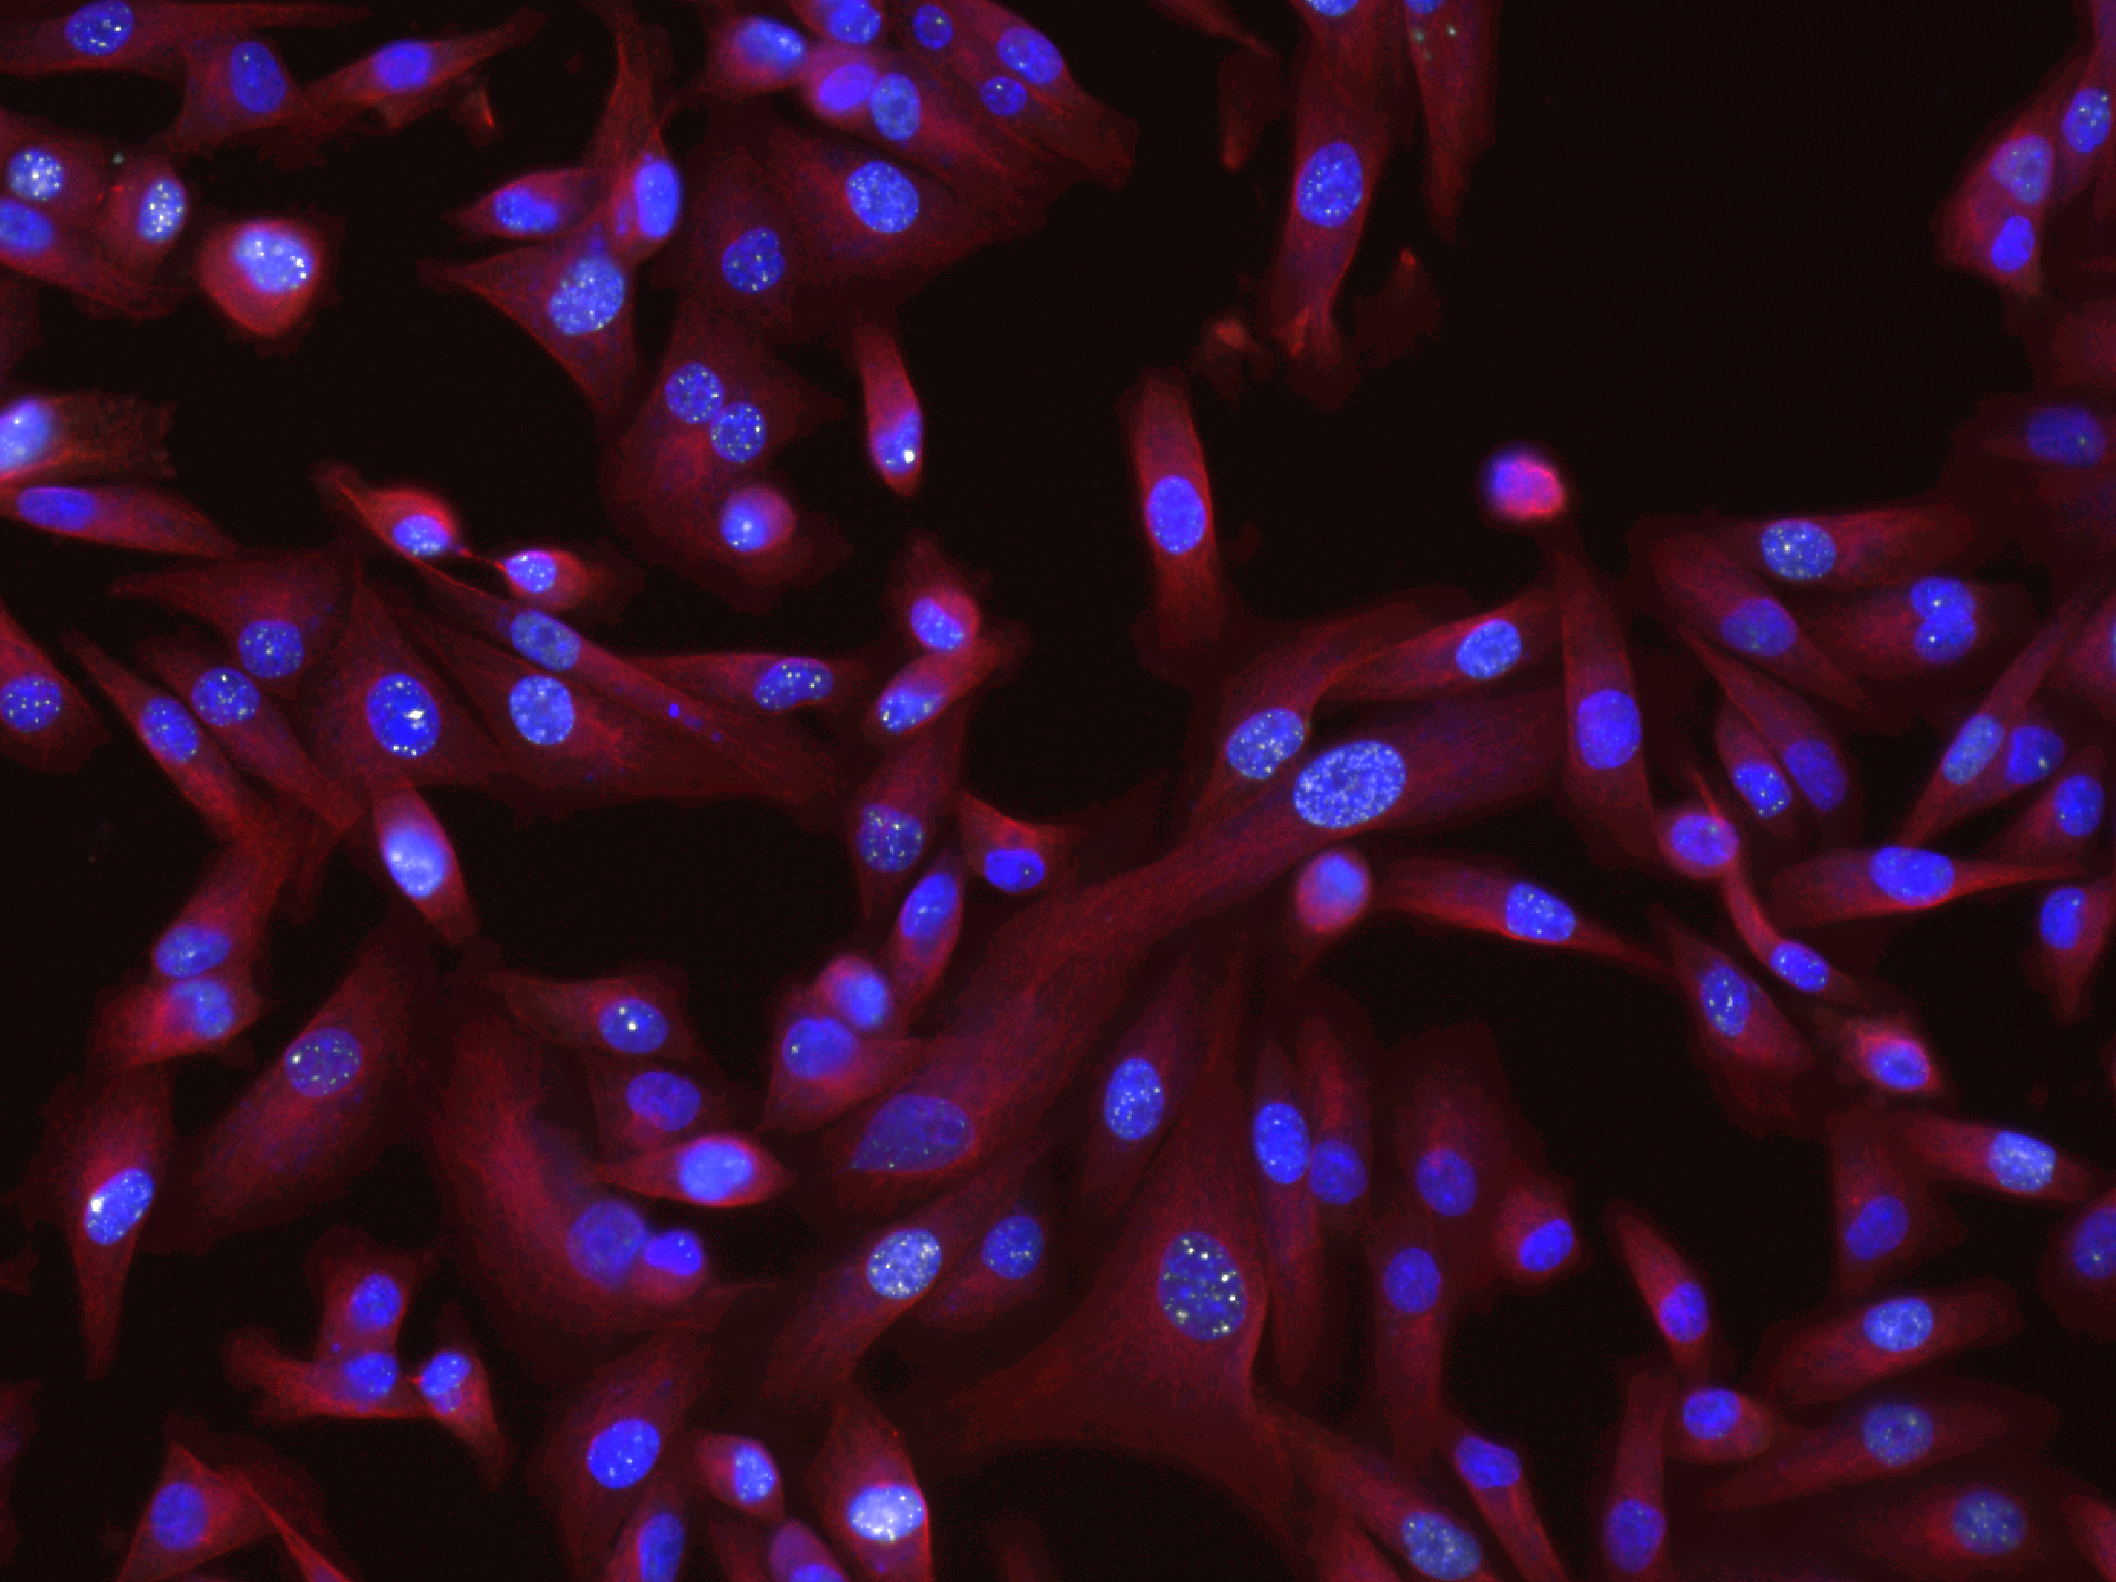
\includegraphics[width=0.95\textwidth]{img/channels.png}
\caption{Fluorescence image of MDA231 cells. DAPI highlighting the nuclei in blue, cyanine 5 highlighting the microtubules in red, and cyanine 3 highlighting the double-strand breaks as white spots on the cell nuclei.}
\label{fig:drug_full_fluorescence}
\end{center}
\end{figure}

\section{Cell measurement pipeline}
\label{sec:cell_measurement}

As mentioned in the introductory Section \ref{subsec:HCA}, the basis of high content analysis are the \emph{features} measured on individual cells. The conventional path to measuring cellular features entails an initial segmentation of individual cells. This section describes the segmentation strategy as well as the features extracted for both the drug and wild type screen datasets described above. These procedures underpin standard preliminary analyses of the data (Section \ref{sec:use_cases}), as well as the developments described in later chapters.

%In our drug screen, the final segmentation yields $122307$ cells for cell line MDA231 and $97134$ cells for cell line MDA468, over $384$ microplate wells each, whereas for our wild type screen we obtain $36338$ cells over $96$ wells.

\subsection{Nuclei segmentation}

The cell nucleus is the logical starting point for cell segmentation (see Figure \ref{fig:segmentation}). Roughly speaking, most nuclei are visible, uniformly-sized, and ellipsoidal, and, crucially, seldom overlap, as the cell surrounding cell membrane acts as a buffer to other cells, and as the cell density has been chosen such that cells do not grow on top of each other. As a result, they are typically the easiest thing to accurately segment in the fluorescent stack, and may then be used as the starting point for segmenting other cytological components. The segmentation typically follows three stages: pre-filtering, detection, and refinement.

\begin{figure}[ht]
\centering
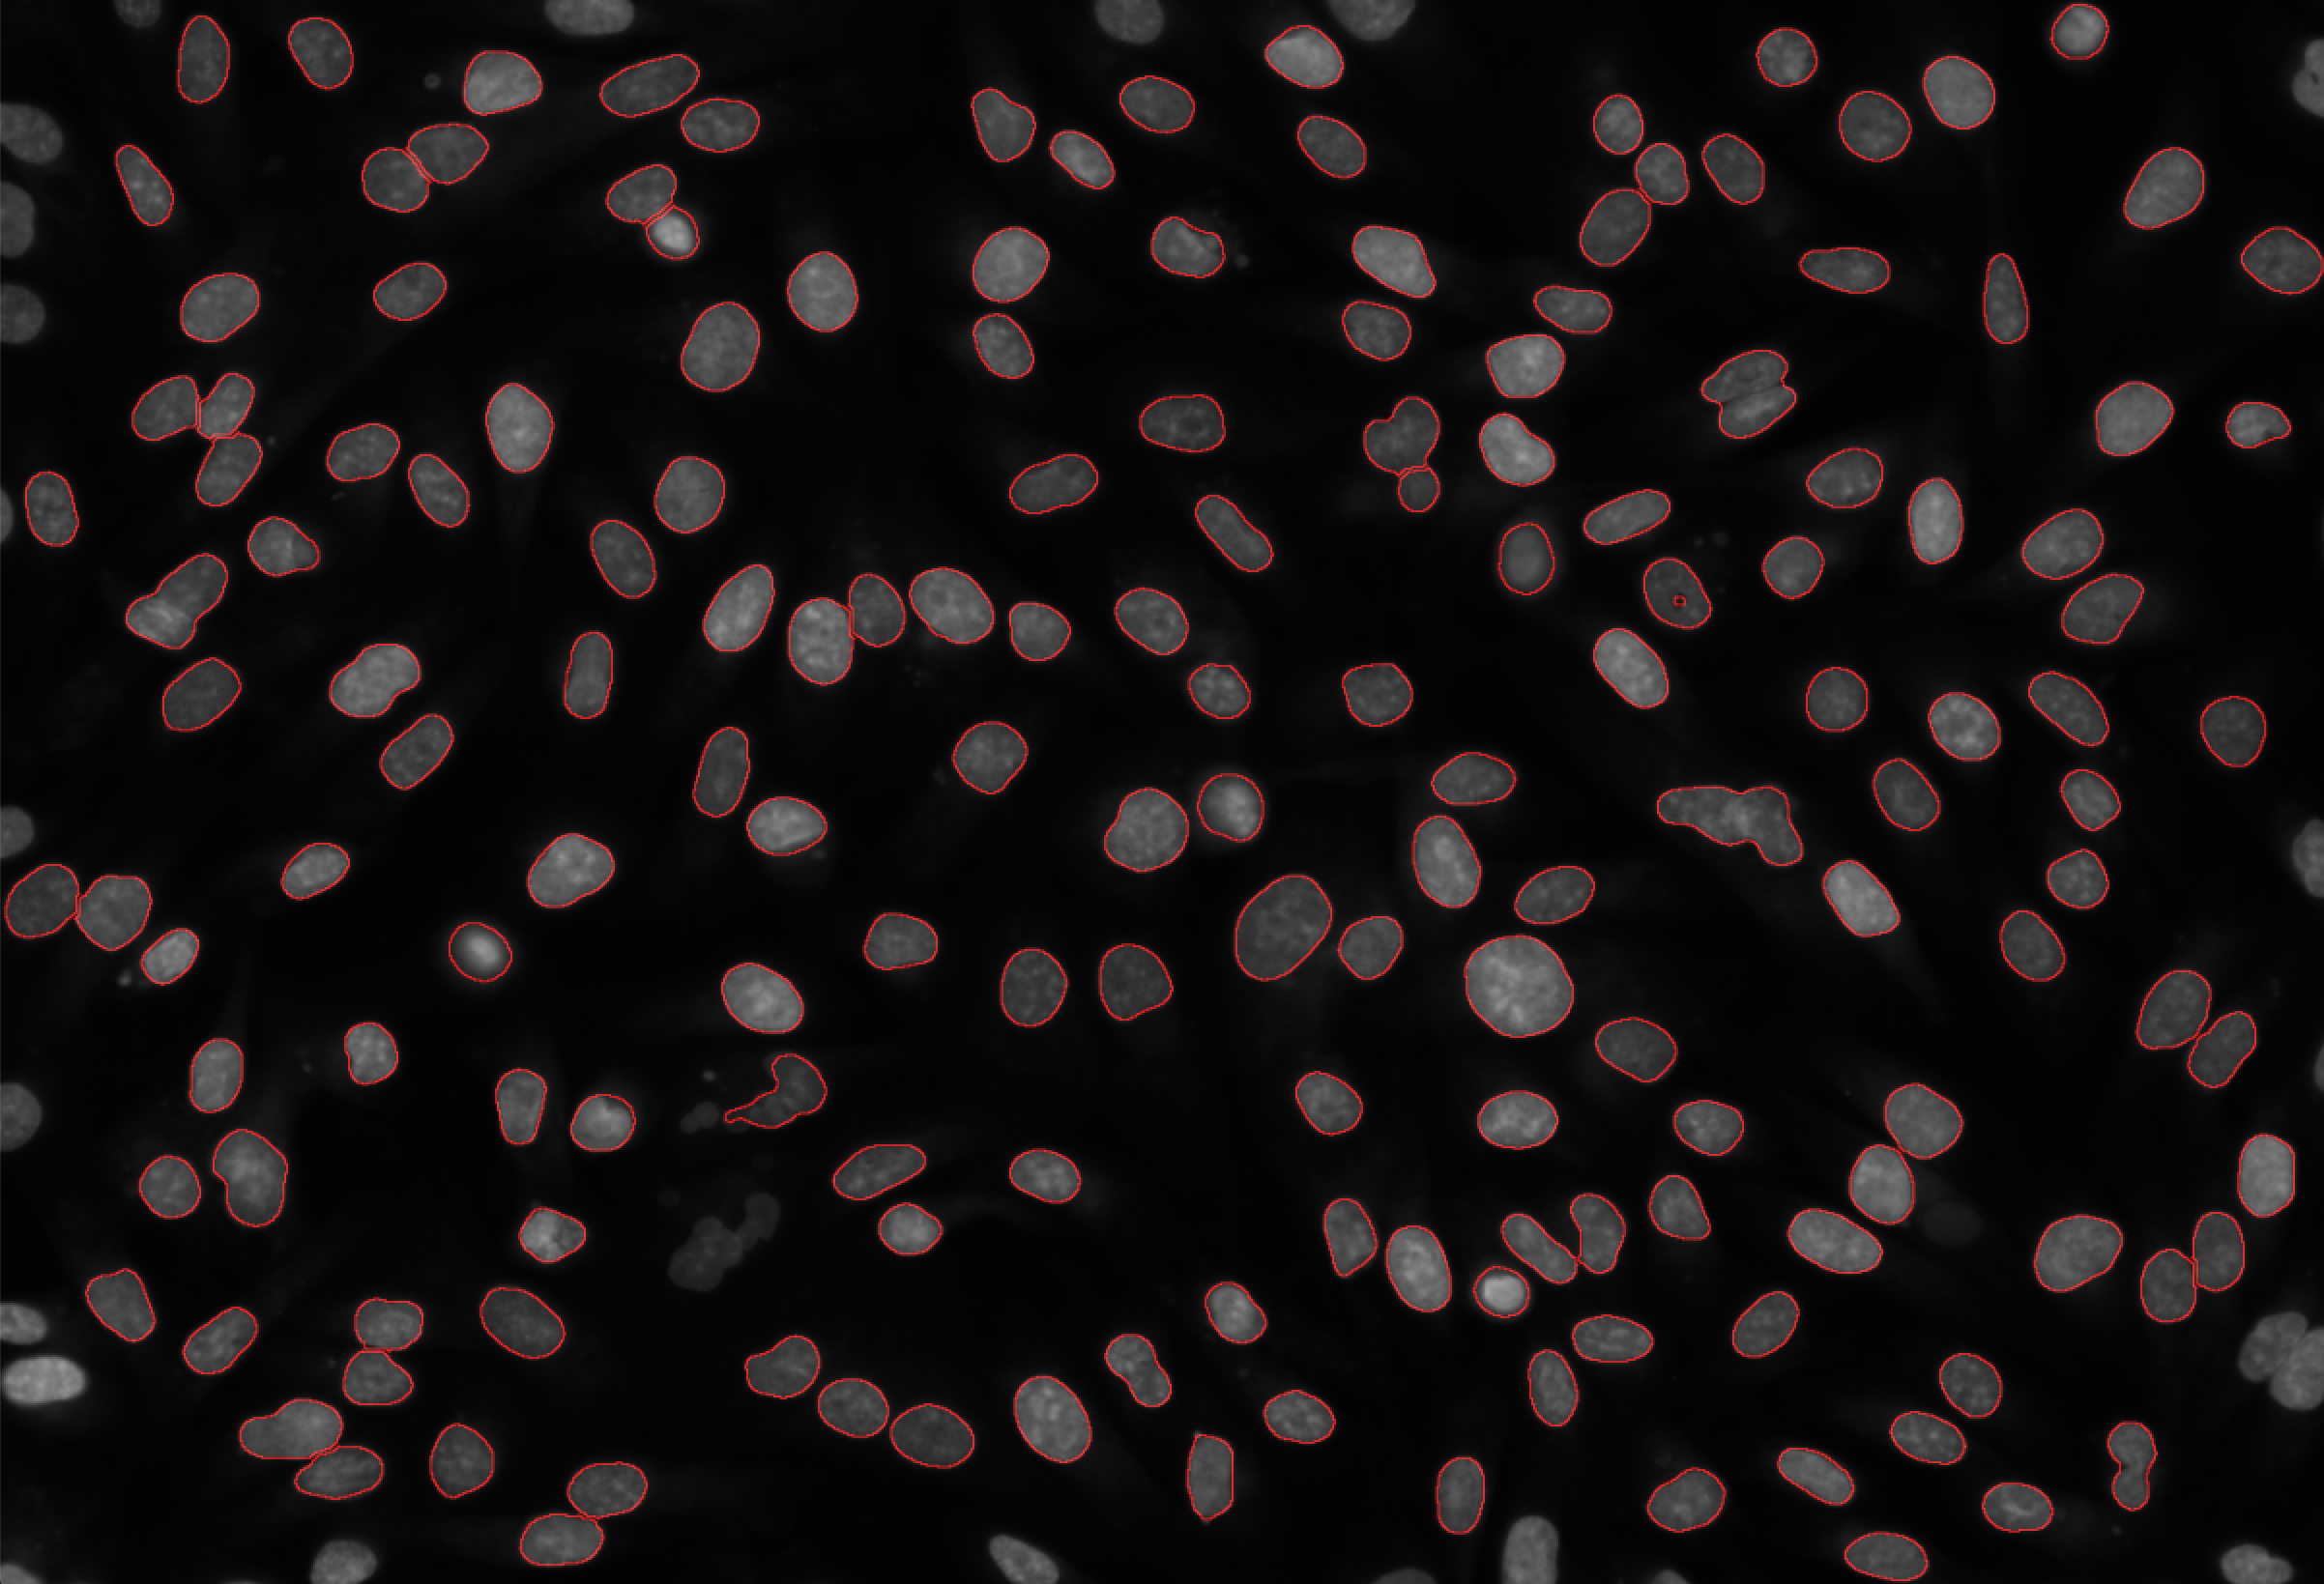
\includegraphics[width=0.95\textwidth]{img/segmentation.png}
\caption{Nuclei segmentation on the DAPI channel, with segmentation contours indicated by red bands.}
\label{fig:segmentation}
\end{figure}

\subsubsection{Pre-filtering}

A common approach to pre-filtering is median filtering (\cite{huang1979fast}), which can be very effective in eliminating noise. The approach works as a sliding window over the image. Thus, for image $f: (X \times Y) \to V$ and window $W(x, y)$ centered on $(x, y)$ of size $m\times n$, one creates a pre-filtered image $p$ with,

\begin{equation}
p(x, y) = \text{median}\{f(x', y') | (x', y') \in W(x, y)\}
\end{equation}

Note the median is an appropriate operator to use as it is robust to outliers, unlike the mean. Note, however, that the elimination of noise may come at the cost of linking separated objects as, depending on the size of the filter, the pixels between nearby objects can be interpreted as outliers.

\subsubsection{Background subtraction}

In order to detect the contours of the cell nuclei, one takes the pre-filtered image $p$ and performs a background subtraction. This again works with a sliding window, $W$, of size $m\times n$, which calculates the local mean intensity for a pixel $b(x, y)$, giving,

\begin{equation}
b(x, y) = \frac{1}{mn}\sum_{i = -\lfloor m/2\rfloor}^{+\lfloor m/2\rfloor}\sum_{j= -\lfloor m/2\rfloor}^{+\lfloor m/2\rfloor} p(x +i, y + j)
\end{equation}

with which one can perform the subtraction yielding,

\begin{equation}
r(x, y) = \max(0, p(x, y) - b(x, y))
\end{equation}

Note that values in $r$ will now be close to zero, with non-zeros corresponding to regions of high intensity gradient. One can therefore identify the contours of the cells, $c(x, y)$ by applying a threshold $t$ giving,

\begin{equation}
c(x, y) = \mathbbm{1}\{r(x, y) \geq t\}
\end{equation}

The nuclei contours may be filled to produce a final segmentation mask.

\subsubsection{Refinement}

In the ideal case of well-separated cells, the aforementioned procedures might be sufficient for perfect nuclei segmentation. However, in practice, some additional steps are required to segment overlapping cells. One of the most classical and widely used refinement approaches is the \emph{watershed} algorithm (\cite{beucher1979use}) applied to the inverse distance map of the segmentation result\footnote{The distance map is the image formed by the distances of the shortest path to the background for every foreground pixel in a segmentation mask.}. Informally, the watershed algorithm simulates a flooding of the topography of the intensity levels in an image. The meeting points of the growing regions build the \emph{watershed line}, which is amounts to a separating line between objects. This method partitions the initially identified object into as many regions as there are local minima of the inverse distance map. In order to avoid over-segmentation due to small irregularities in the object boundary potentially leading to local minima, one selects local minima according to their morphological dynamic (\cite{Grimaud1992}).

\subsection{Cell membrane segmentation}

With the cell nuclei segmented on the DAPI channel, one proceeds to segment the cell cytoskeleton, approximated by the microtubules on the Cy5 channel. Here we follow the approach of \cite{jones2005voronoi}, which uses the cell nuclei as seeds for the more difficult cell membrane segmentation. The approach consists of defining a specialised distance metric that accounts for changes in intensity (high gradients), with the matrix,

\begin{equation}
\mathbf{G} = \begin{bmatrix}
(\frac{\partial g}{\partial x})^2 & \frac{\partial g}{\partial y}\cdot\frac{\partial g}{\partial x}\\
\frac{\partial g}{\partial x}\cdot\frac{\partial g}{\partial y} & (\frac{\partial g}{\partial y})^2
\end{bmatrix}
\end{equation}

where $\mathbf{g}(\mathcal{I})$ is Gaussian blur, whose gradients are simply the finite central difference of the adjacent pixels (these too can be defined by convolutions), and infinitesimal distances are calculated as,

\begin{equation}
||d\mathbf{x}||_{\mathbf{G}}^2 = d\mathbf{x}^T\mathbf{G}d\mathbf{x}
\label{eq:infinitesimal}
\end{equation}

In reality, we have,

\begin{equation}
G = \frac{\nabla g(f)\nabla^Tg(f) + \lambda I}{1+\lambda},
\end{equation}

hence the distance between two points is given by the compromise between gradient based distance and Euclidean distance,

\begin{equation}
dx^TGdx = \frac{\|dx^T\nabla g(f)\|^2 + \lambda\|dx\|^2}{1+\lambda}
\end{equation}

The distance metric is defined for neighbouring pixels. Distances between non-adjacent pixels are computed as the shortest path (for example with Dijkstra's algorithm). Thus, the metric behaves like a spatial distance metric on flat, uniform regions, yet takes intensity into account where necessary. The segmentation is performed by assigning pixels to the nearest seed, that is, cell nucleus, under this Euclidean-regularised metric. One may see from Equation \ref{eq:infinitesimal} that the metric converges to Euclidean distance as $\lambda \to \infty$. Hence, the segmentation becomes a Voronoi tesselation in the limit. 

The tunable parameters of the algorithm are: the size (receptive field) of $g\mathcal{I}$; an initial global thresholding step to eliminate the background, for example with an Otsu threshold (\cite{otsu1979threshold}); and the regularisation $\lambda$.

\subsection{Feature extraction}

In order to quantify cellular phenotypes, features are extracted from the segmented cells. These features can be interpretable or general shape, intensity and texture descriptors. In this base line approach, I used the features provided by standard open-source software tools, here CellCognition\footnote{http://cellcognition-project.org}. Cell Cognition can export many hundreds of features for each fluorescent channel at the user's discretion. These features generally fall into the following categories: basic intensity features, basic shape features (e.g. RoI size, perimeter, circularity), convex hull features, distance map features, granulometry features, Haralick features, moments, and statistical geometric features (see \cite{held2010cellcognition, walter2010automatic} for a detailed description). 

%\subsubsection{Haralick features}
%
%Haralick or gray level co-occurrence matrix (GLCM) features (\cite{haralick1973textural}) are used in image analysis as a measure of texture. One computes the matrix $\mathbf{H}$ where the element $\mathbf{H}(i, j)$ is equal to the number of times grayscale level $i$ and grayscale level $j$ (usually from an $8$-bit range) co-occur at a chosen offset $(\delta x, \delta y)$. The matrix is then reduced to a set of summary statistics (the features), such as correlation and entropy.

In these experiments, 238 features were extracted for each of the DAPI and Cy5 channels, and 38 for the Cy3 channel, giving 516 features in total for each cell. These features are engineered to be plausibly discriminative, yet rarely have an immediate biological sense. Nevertheless, a minority of features can inform about some basic biological phenomena: the size of each segmented object (RoI size) on the DAPI channel directly quantifies nuclear size, from which one may infer about cell growth and aberrant phenomena such as chromosome segregation problems and consequent micronucleation; granulometry and Haralick features measure texture structures, which can be a proxy for mitochondria; average DAPI intensity can indicate an interphase cell prior to or after DNA replication; and spot features directly measure double-strand breaks (DSBs) on the Cy3 channel (see Section \ref{subsec:multivariate}).

\section{Use cases in high content analysis}
\label{sec:use_cases}

The following section details a series of use cases of explorative analysis in the drug and wild type screens. Section \ref{subsec:spatial_effects} first investigates the possible presence of spatial biases in the drug screen microplates. Sections \ref{subsec:viability} and \ref{subsec:multivariate} in turn describe a univariate and multivariate analysis of the drug screen. Finally, machine learning techniques are used in Section \ref{subsec:tnbc_classification} to make morphological comparisons of TNBC cell lines in their wild type.

\subsection{Controlling for spatial effects in the drug screen dataset}
\label{subsec:spatial_effects}
One concern in HCS is the presence of systematic bias in the experimental setup. Controlling for this bias is the objective of a series of quality control techniques. In the pilot drug screen dataset, with a single plate per cell cell line, the most relevant concern is the presence of \emph{spatial bias}, that is, a dependency of the phenotypic readout on the position of the well on the plate. A common cause of such a bias is a temperature gradient inside the incubator during hibernation. This can result in an uneven evaporation of well solvents, in particular around the microplate borders, leading to an alteration of the drug concentration. Where spatial biases exist, their effects might be corrected for (\cite{Caraus2015, Ljosa2009}). However, the best solution is certainly to reconduct the experiments, as statistical correction only addresses effect strength, not phenotypic alterations (for example, if more cells are dead, one cannot infer what would have happened had the concentration been lower).

%\st{In Section} \ref{subsec:hcs} we discussed the use of the $Z$-factor as a validation for assay quality in high throughput screening. According to \cite{singh2014increasing}, however, the $Z$-factor is at odds with a high content phenotypic screen, as it is defined only for univariate readouts. Systematic biases or \emph{plate effects} are more usually combatted with a smaller number of replicates (four or five according to \cite{bray2016cell}).

\begin{figure}%
    \centering
    \subfloat[MDA231 cell counts]{{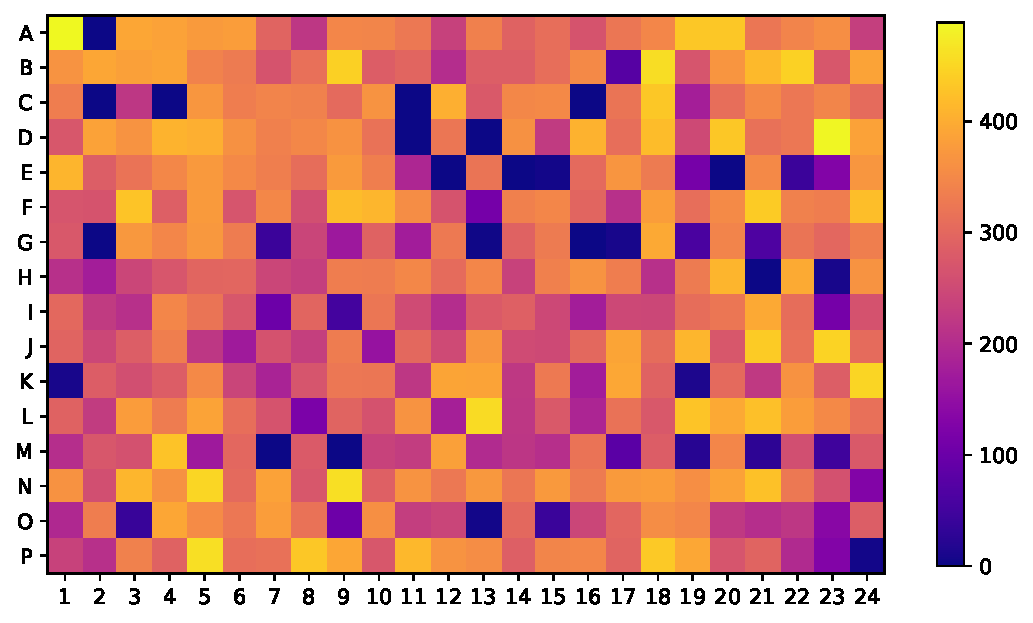
\includegraphics[width=0.45\textwidth]{img/plate_cell_counts_mda231.pdf}}}
    \qquad
    \subfloat[MDA468 cell counts]{{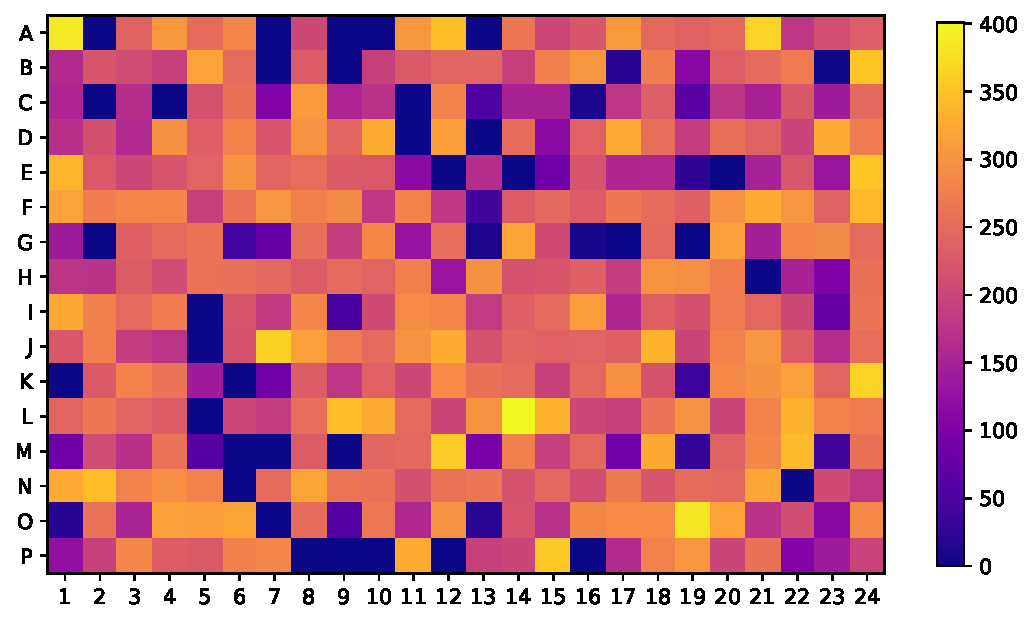
\includegraphics[width=0.45\textwidth]{img/plate_cell_counts_mda468.pdf}}}
    \qquad
    \subfloat[MDA231 PCA1]{{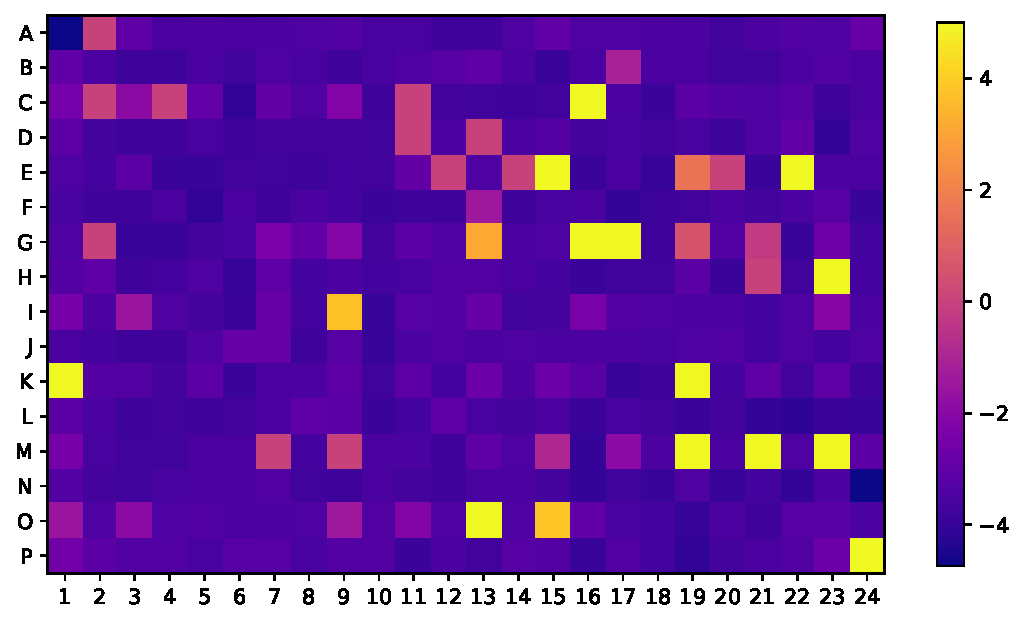
\includegraphics[width=0.45\textwidth]{img/plate_pca1_mda231.pdf}}}
    \qquad
    \subfloat[MDA468 PCA1]{{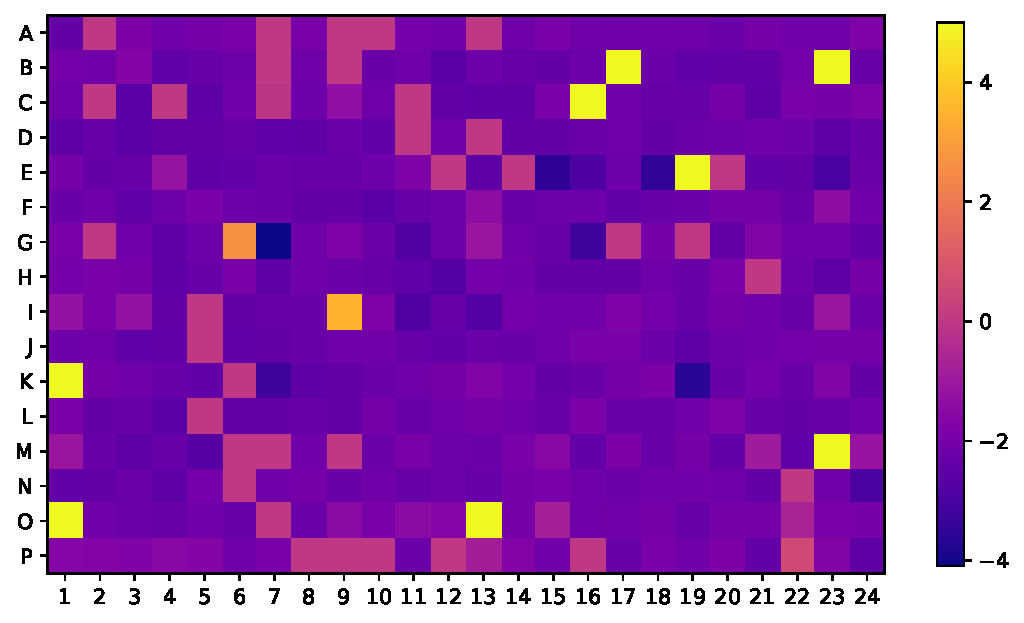
\includegraphics[width=0.45\textwidth]{img/plate_pca1_mda468.pdf}}}
    \qquad
    \subfloat[MDA231 PCA2]{{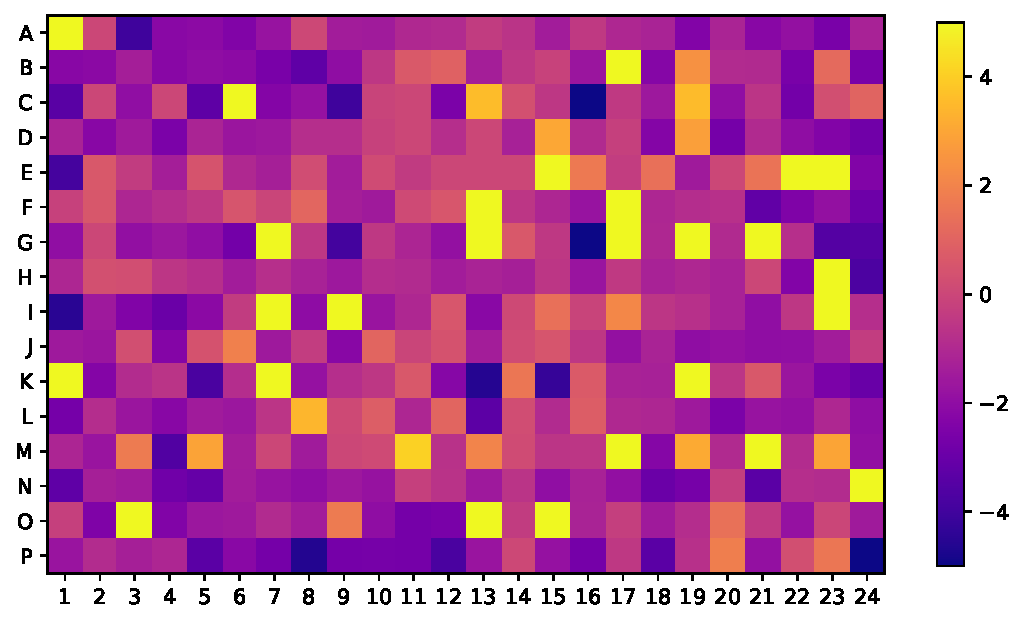
\includegraphics[width=0.45\textwidth]{img/plate_pca2_mda231.pdf}}}
    \qquad
    \subfloat[MDA468 PCA2]{{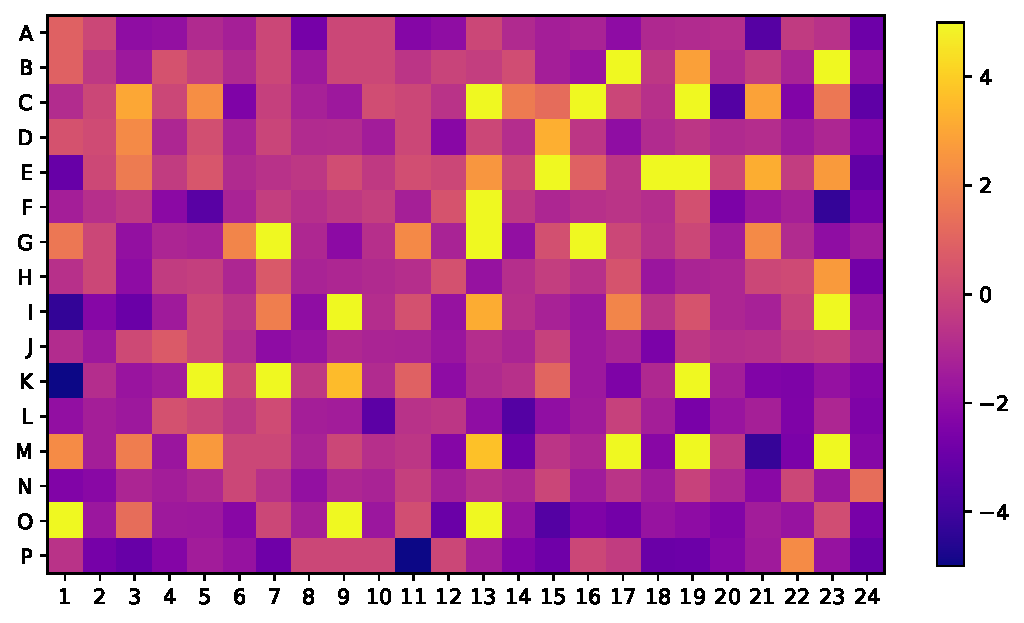
\includegraphics[width=0.45\textwidth]{img/plate_pca2_mda468.pdf}}}
    \caption{Searching for spatial biases: comparison of cell counts (a), (b); comparison of first principal component of morphological profiles (c), (d); comparison of second principal component (e), (f), arranged according to the spatial . Left column (a), (c), and (e) pertain to cell line MDA231; right column (b), (d), (f) to cell line MDA468.}%
    \label{fig:plateeffects}%
\end{figure}

Spatial biases are investigated in Figure \ref{fig:plateeffects}. These figures visualise, for both cell lines, firstly the number of cells in each of the $384$ wells of the plate (indexed first by the alphabetic vertical axis, then by the horizontal numeric axis). The cell count relates directly to viability, a key readout for drug potency. Also visualised are, in turn, the first and second principal components of the matrix formed from the vectors of mean feature readouts for the cells of each well. Note that these vectors amount to a simple phenotypic profile of the well condition (a construct that will be explored in great detail in Chapter \ref{Chapter4}). The principal components of the profile matrix (taken separately) therefore provide a univariate summary of phenotypic information for each well. Small clusters appear in each heat map reflecting the clustering of similar negative controls, however there is no apparent border effect or directional tendency that would indicate systematic bias for any of the three readouts. The validity of the screen data may therefore be concluded.

\subsection{Viabilities of TNBC cell lines correlate}
\label{subsec:viability}

\begin{figure}
\centering
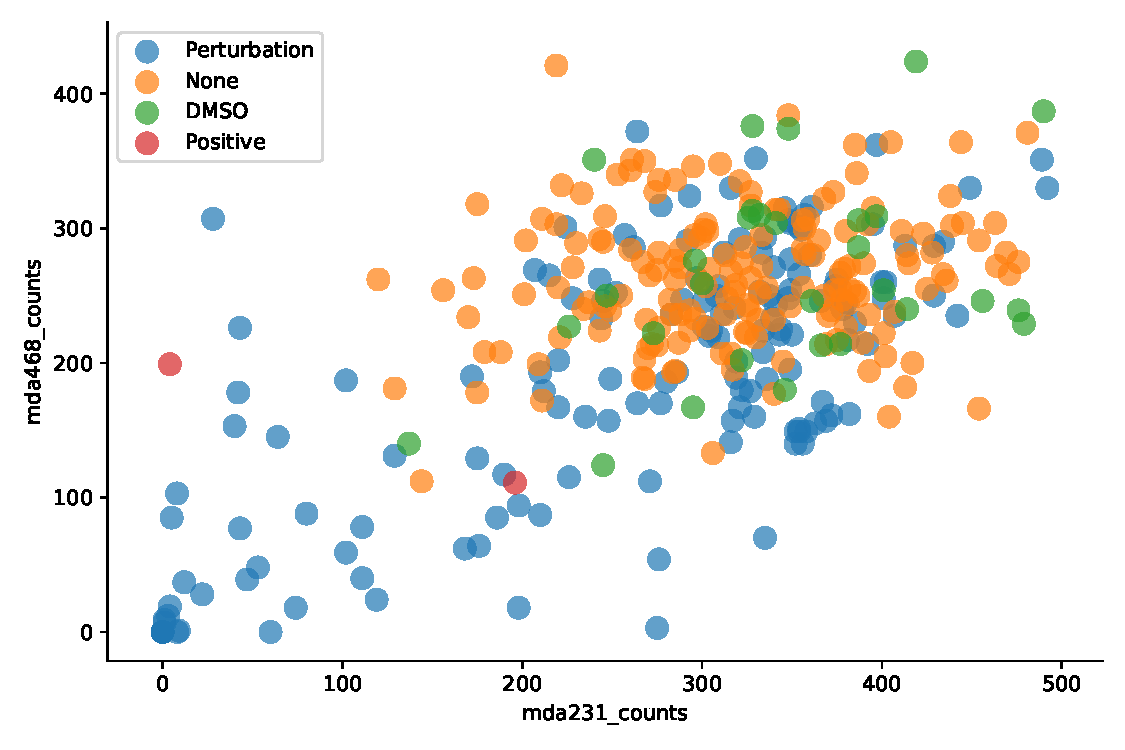
\includegraphics[width=0.85\textwidth]{img/viability.pdf}
\caption{Viability comparison between cell lines for a variety of drugs and negative controls. The neutral DMSO and untreated wells strongly overlap, while showing considerable variation in both cell lines. Viability correlates well between cell lines with Pearson correlation coefficient $\rho = 0.6556$}
\label{fig:viability}
\end{figure}

\begin{figure}%
    \centering
    \subfloat[Calcineurin inhibitors]{{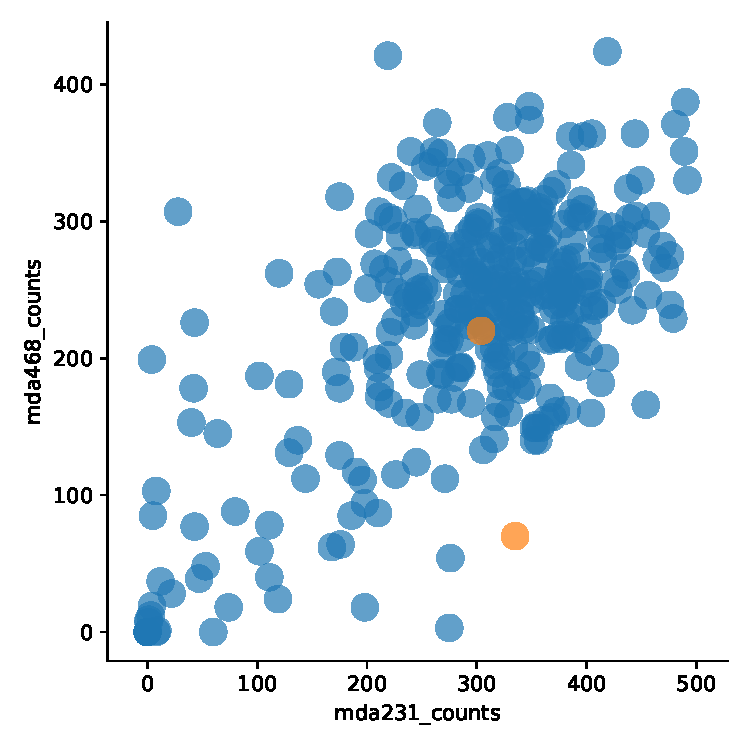
\includegraphics[width=.45\linewidth]{img/viability_Calcineurin_Inhibitor.pdf}}}%
    \qquad
    \subfloat[DNA damage (positive)]{{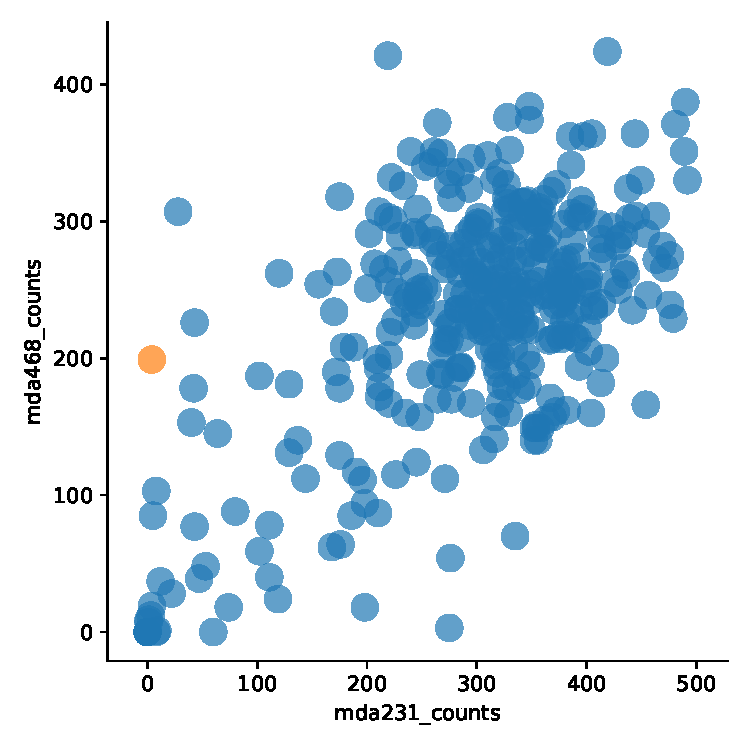
\includegraphics[width=.45\linewidth]{img/viability_DNA_Damage.pdf}}}%
    \qquad
    \subfloat[CDK inhibitors]{{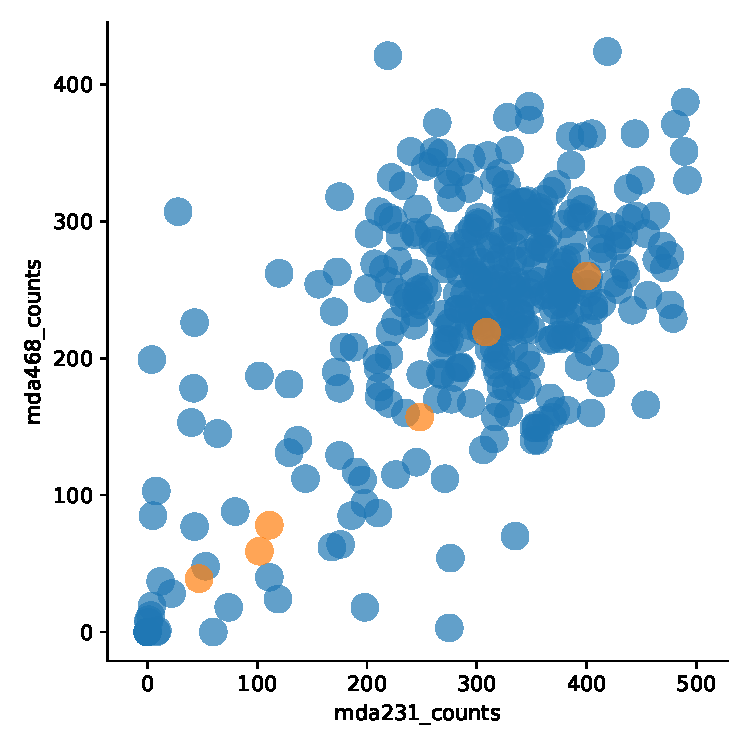
\includegraphics[width=.45\linewidth]{img/viability_CDK_Inhibitor.pdf}}}%
    \qquad
    \subfloat[MMP inhibitors]{{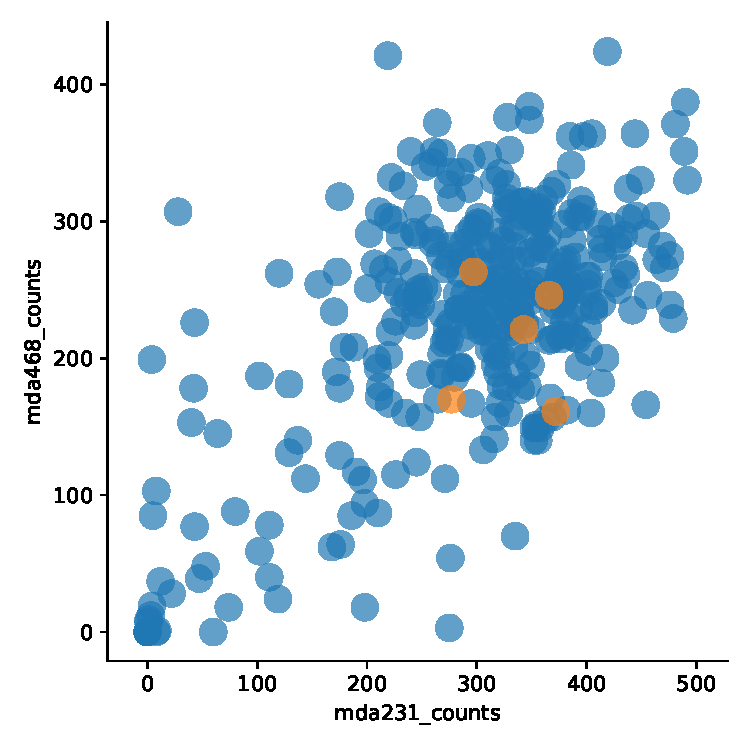
\includegraphics[width=.45\linewidth]{img/viability_MMP_Inhibitor.pdf}}}%
    \qquad
    \subfloat[PKC inhibitors]{{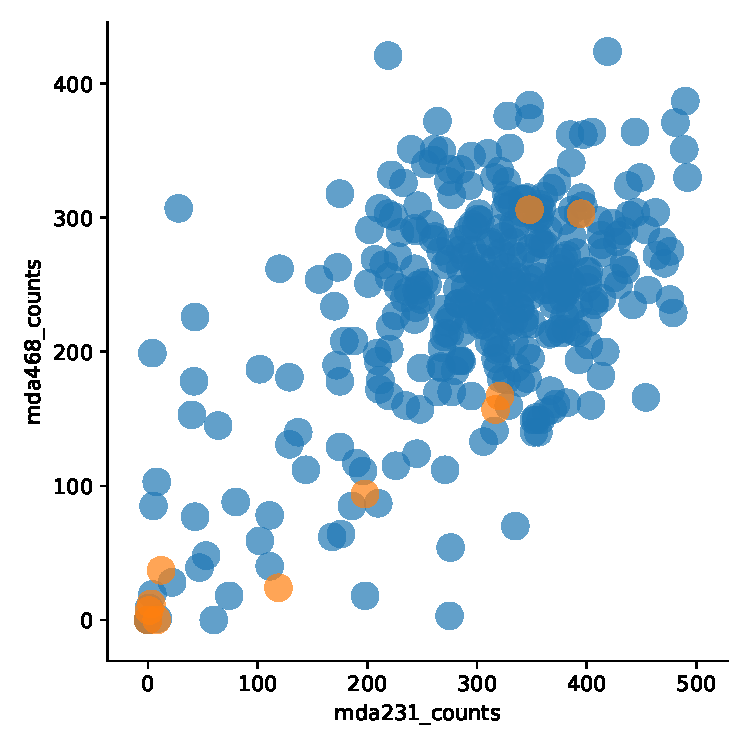
\includegraphics[width=.45\linewidth]{img/viability_PKC_Inhibitor.pdf}}}%
    \qquad
    \subfloat[Tyrosine kinase inhibitors]{{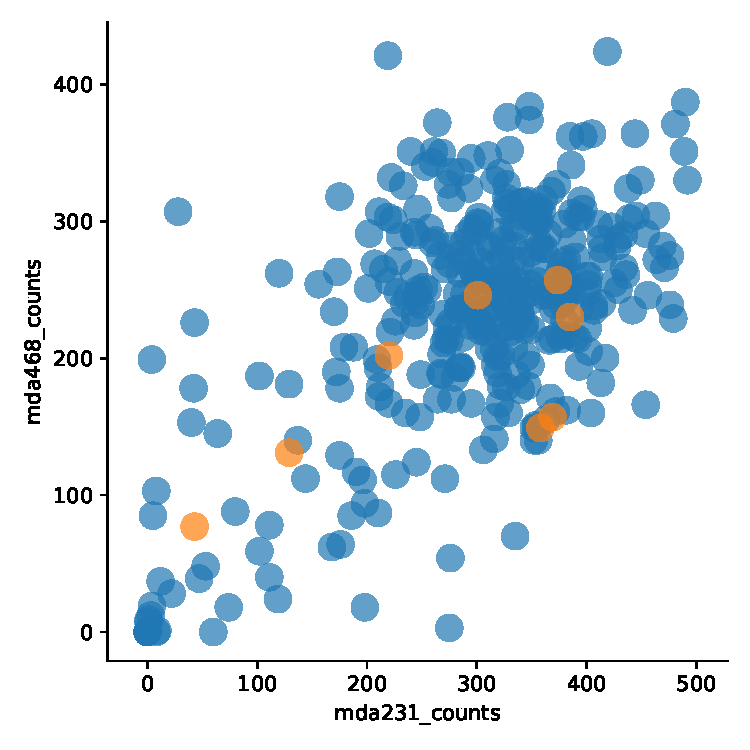
\includegraphics[width=.45\linewidth]{img/viability_Tyrosine_Kinase_Inhibitor.pdf}}}%
\caption{Comparison of viability by drug mechanism of action. One may observe differential effects by cell line: (a), (b) show differential effects on viability; (c) shows no clear divergence from the control cluster; (d), (e), (f) show a range of correlated effects.}
\label{fig:viability_moas}
\end{figure}

One of the initial aims of this TNBC pilot drug screen is simply to quantify cell \emph{viability}. In a viability assay, viability is conventionally measured in the range [0, 1] (\cite{pegg1989viability}). Given that cells are seeded at a fixed density, the change in the number of dead cells with respect to the negative control is an indication of the viability. The viability,

\begin{equation}
v = \frac{n^d}{n^-}
\end{equation}

of cells in response to a drug $d$ refers to the change in the population size $n^d$ relative to that of the negative control $n^-$. Due to the effects of \emph{lysis} (cellular breakdown) and the washing procedure, the cells remaining at the point of imaging are the ``survivors'' of the drug perturbation. When cells are segmented, the viability of a drug is given by the cell sample size. When cells are not explicitly segmented, the viability is represented indirectly by how populated the field is. Viability is an important phenotypic characteristic of a drug effect. In Figure \ref{fig:viability} we are able to compare the number of segmented cells (therefore a proxy viability) between well populations of cell lines MDA231 and MDA468 subjected to the same perturbations. The majority of viabilities belong to a dense cluster of negative controls (\emph{DMSO} and \emph{None}) with an average of $289$ cells for cell line MDA231 and $227$ cells for MDA468. We additionally observe a small cluster of highly potent cytotoxic drugs near the origin. There is a positive correlation of $\rho = 0.6556$ for the viability of the two cell lines, suggesting that in many cases, one can actually expect a similar viability phenotype for both cell lines. However, a closer look at Figure \ref{fig:viability} shows that this is by no means true for all drugs. Some drugs act differentially on both cell lines, demonstrating the heterogeneous effect on distinct molecular TNBC subtypes discussed in section Section \ref{subsec:multi_cell_line_data}. These \emph{differential drug effects} correspond to the ``L''-structure traced by the data points skirting the horizontal and vertical axes of the plotting area.

This comparison furthermore allows us to categorise drugs as having no effect, joint effect, or separate effects on the two cell lines. Figure \ref{fig:viability_moas} visualises the same population data, this time coloured by selected drug mechanism of action (MOA) categories. We see, in particular, the success of protein kinase C (PKC) inhibitors in regularly killing most--if not all--cells in both cell lines, with a small cluster nearby the origin. Note that PKC inhibitors induce interesting phenotypes under other modes of analysis, as we shall see in both Section \ref{subsec:multivariate} and Section \ref{subsubsec:differential}.

\subsection{Cell cycle modulates double-strand break rate}
\label{subsec:multivariate}

\emph{This section contains an excerpt from a paper published in at the International Symposium for Biomedical Imaging in 2018. The paper is reproduced in full in Appendix \ref{AppendixD}.}

An example of multivariate analysis in the assay arises in the analysis of double strand breaks (DSBs). Dysfunction of the DNA repair mechanisms is a major hallmark of cancer, also providing therapeutic opportunities. Monitoring DNA damage by the fluorescent labeling of double strand breaks (DSB) in cells is therefore an important readout in drug screening of cancer cell lines. DSBs occur when both strands of the DNA double helix are broken. DSBs have various causes, for example, cytotoxic radiation, or DNA replication over an existing single-strand break. Despite the natural DNA repair mechanisms of the cell, DSBs can be irreparable, leading ultimately to apoptosis, or hazardous DNA rearrangements. As such, DSBs are an interesting property to assess when analysing the effects of small compounds upon cancer cells. Three approaches to quantifying DSBs on the Cy3 fluorescence channel are compared, based on detecting and counting spots, granulometric features, and average intensity, which are mutually strongly correlated readouts.

\begin{figure}[h!]%
    \centering
    \subfloat[\label{fig:dsb_figure_a}]{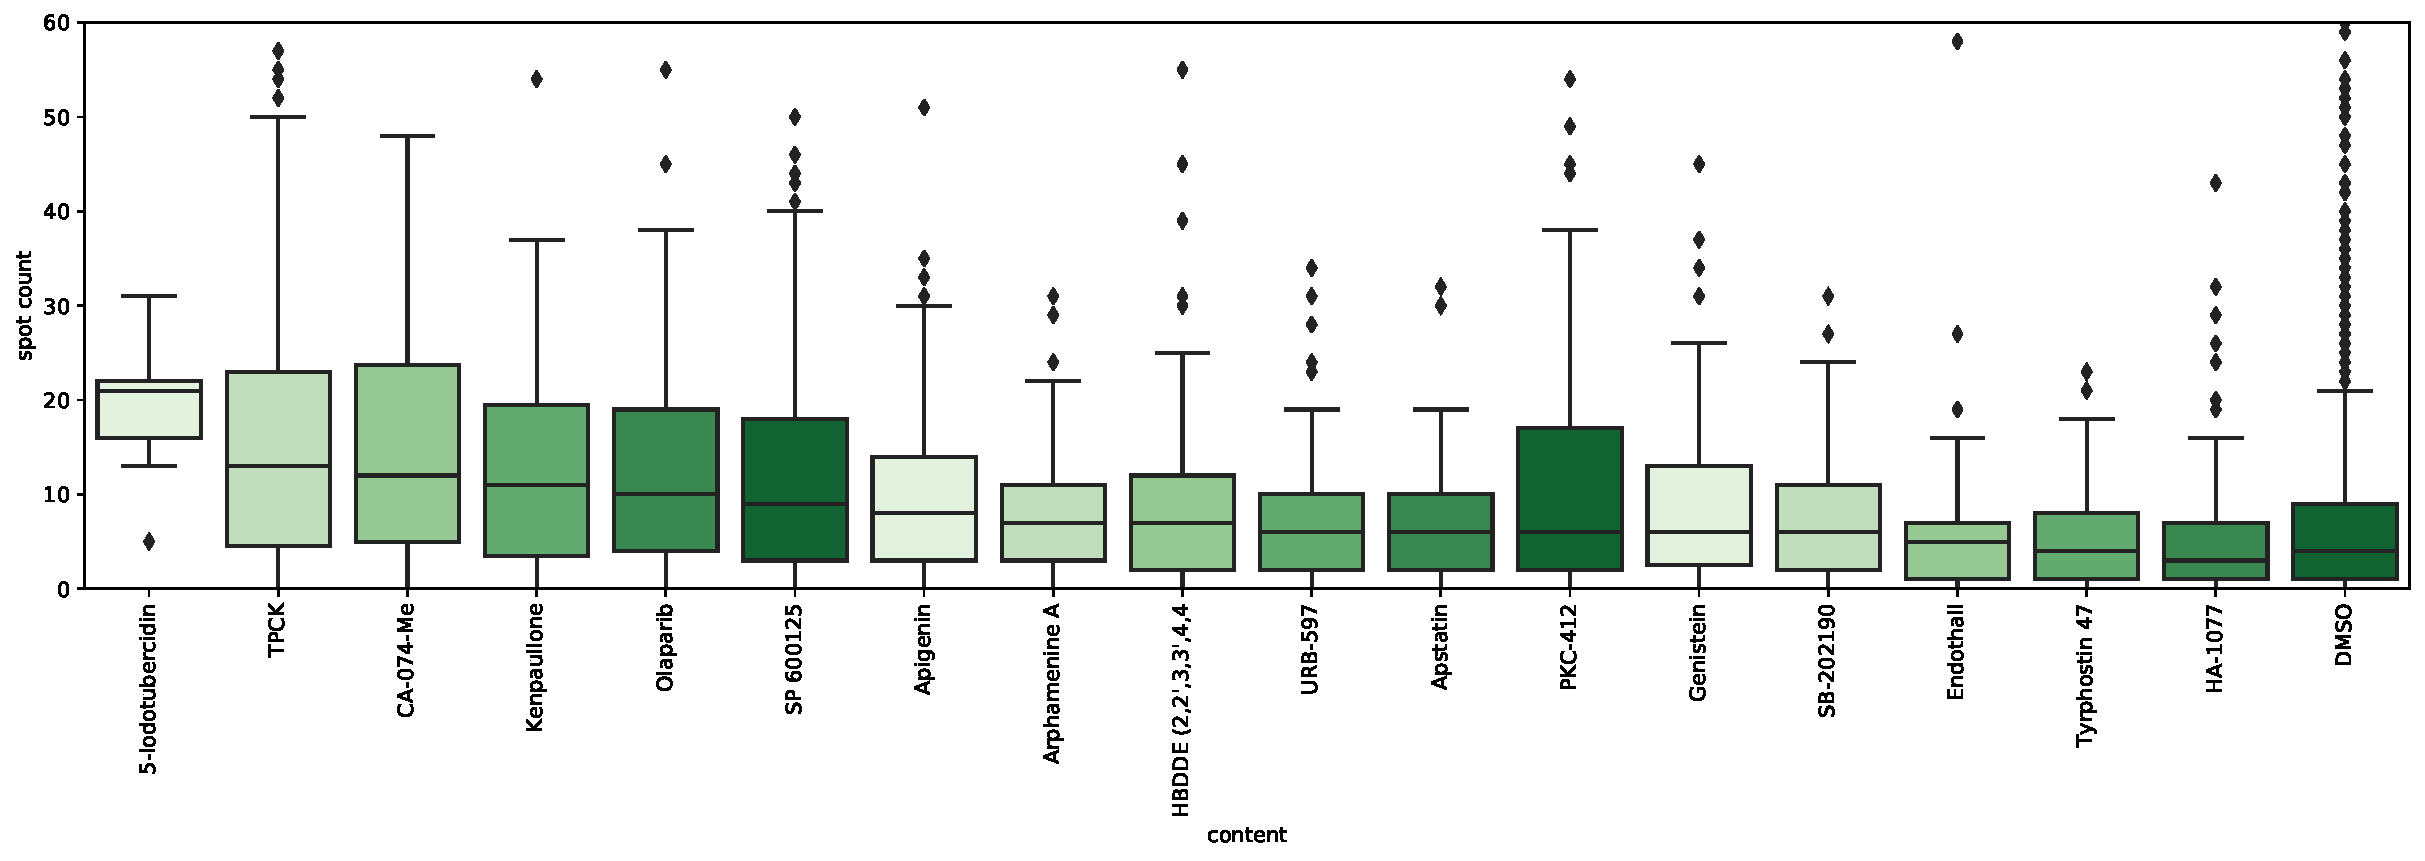
\includegraphics[width=\textwidth]{img/dsb_box_plot.pdf}}
    \qquad
    \subfloat[\label{fig:dsb_figure_b}]{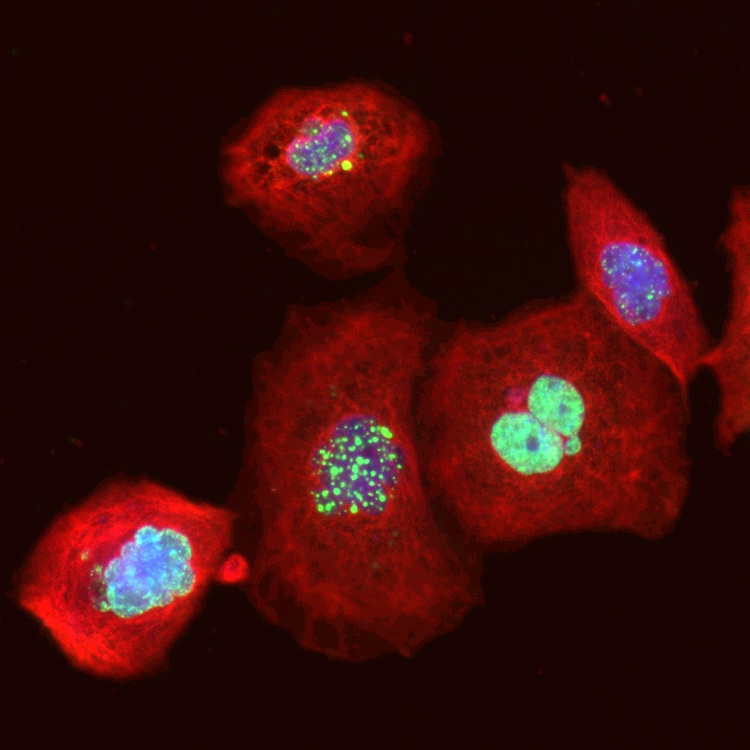
\includegraphics[width=0.45\textwidth]{img/dsb_pkc412.png}}
    \qquad
    \subfloat[\label{fig:dsb_figure_c}]{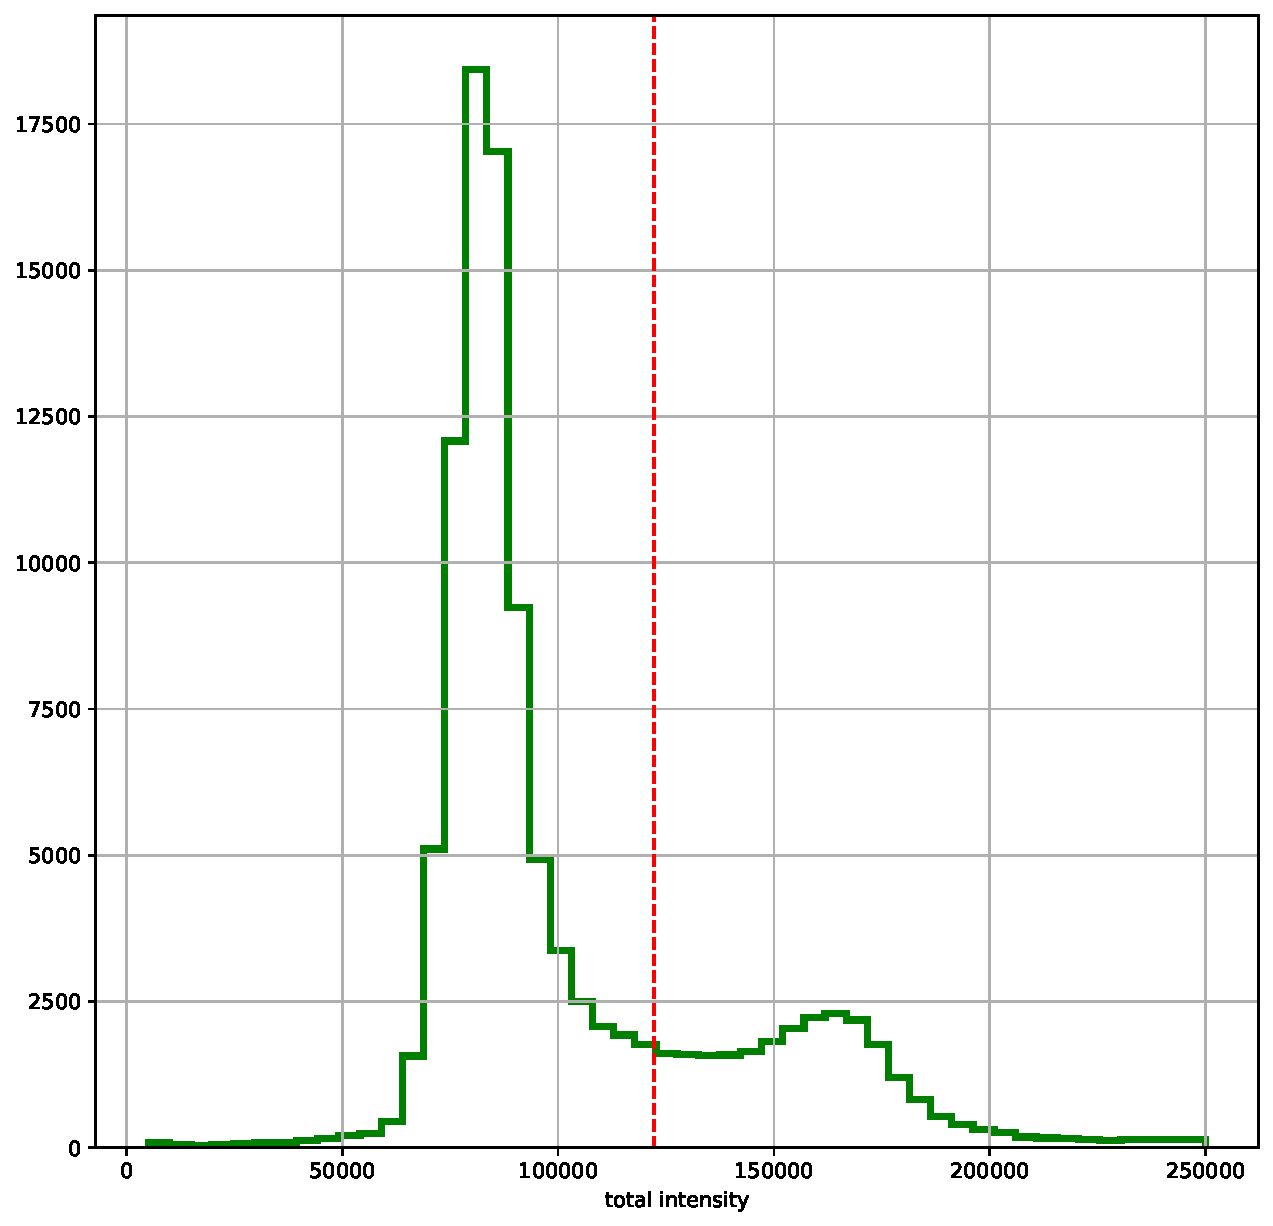
\includegraphics[width=0.45\textwidth, width=0.45\textwidth]{img/dsb_otsu.pdf}}
  \caption{Drug perturbations inducing significant changes to DSB distribution (measured by spot density) on cell line MDA231 at $p = 0.01$ with multiple testing correction, ordered by median spot density. Sample of cells perturbed with significant drug PKC-412 (b), DSBs visible as green spots above nucleus. A bimodal distribution is seen on the DAPI channel revealing a growth of mean intensity post DNA replication (c). An Otsu threshold (red vertical line) can be used to stratify the cell population, further revealing distributional differences in DSB rates.}
\label{fig:dsb_figure}
\end{figure}

\emph{Spot density} (spot count normalised by nuclear size) is used as the basis of a DSB comparison between perturbations and negative control. The distribution of spot density from a perturbation is compared with that of the negative control in a Kolmogorov-Smirnov (KS) test. Hits are declared at a $p$-value of $0.01$, with multiple testing controlled for with a Benjamini-Hochberg correction. Significant results are displayed in Figure \ref{fig:dsb_figure_a}, ranked by median spot density and a sample of cells from a significant drug PKC-412 are shown in \ref{fig:dsb_figure_b}. 

Although some drugs have a clear effect on DSBs, they might also cause intermediate effects, which themselves modulate DSB rates. We see in Figure \ref{fig:dsb_figure_c} a bimodal distribution in fluorescent density on the DAPI channel, apparently reflecting subpopulations of cells in the G$_1$ and G$_2$ phases of the cell cycle. The higher frequency of low intensities corresponds to the longer G$_1$ phase meaning more cells will be fixed in this phase after hibernation. Because S phase (DNA replication) occurs between the G$_1$ and G$_2$ phases, there is more DNA available on which DSBs can occur.  Controlling for these phases produces different distributions of DSBs in the G$_1$ and G$_2$ subpopulations. This multivariate analysis thus reveals an \emph{effect modifier} of cell cycle phase on DSBs. Stratification is used to establish whether increased rates of DSBs are a direct effect of perturbation or an indirect effect of a modified cell cycle. See Appendix \ref{AppendixD} for further detail.

PKC inhibitors are found to feature prominently among the drugs inducing highest spot densities per cell. However, we know from Section \ref{subsec:viability} that drugs in this MOA category often cause low viability. Populations with low sample size tend not to meet the significance criteria. It is therefore drugs such as PKC-412 (Figure \ref{fig:dsb_figure_b}), which kill fewer cells, that are ultimately declared as hits. Thus, we may identify a potential selection bias: DSBs are a cytotoxic effect that, when induced at a high rate by perturbation, should increase the rate of cell death. Given the experimental protocol, dead cells are not fixed and are lost during the fluorescence washing step. Hence, the more severe the drug effect on DSBs, the fewer the cells available for measurement. It is concluded in Appendix \ref{AppendixD} that this systematic bias cannot be resolved from the available data, and can only be avoided in future assays with an adjusted imaging protocol, but it points to potential problems in the interpretation of the derived hit list.

%shows that interpretation of hit lists calculated from univariate features is to be taken with care

In this section, it has been shown that even in the case that one is interested only in a single feature (here the number of DSBs or a surrogate feature), it is still beneficial to use a multivariate readout in order to extract a better understanding and a cleaner analysis. In addition, the causal inference framework has been used in order to correct for confounding variables. Given that the analysis of DSBs is very widely used in the field of cancer drug screening, it is important to alert the scientific community to potential misinterpretations of their screening results.

%\subsection{Machine Learning for HCA}
%
%Machine learning performs inference freely on large numbers of variables. Though this is still a sort of multivariate analysis, we are no longer necessarily restricting the analysis to interpretable variables. Instead, we may analyse the statistical tendencies of complex feature aggregations. The biological meaning may, however, be instilled by other means, as we shall show in the following two use cases.

\subsection{TNBC cell lines assume distinct wild type morphologies}
\label{subsec:tnbc_classification}

At a glance, one can see that TNBC cell lines manifest distinct morphologies, even in the absence of perturbation. To better understand the degree of this difference, we turn to the wild type screen on $12$ cell lines ($11$ TNBC + negative control). The segmentation and feature extraction pipeline detailed in Section \ref{sec:cell_measurement} is used. With each cell described by a vector of features, one may proceed to aggregate the readouts so as to describe the cell population in a similar way. Such a phenotypic profile can, for example, summarily characterise the response of the cell population to a given drug perturbation. Profiles, comprising of vectors of aggregated features, can then serve as the basis of comparison between drug effects on a cell line. While this methodology is explored in detail in Chapter \ref{Chapter4}, here let us consider the special case where individual cell phenotypes are identifiable by an expert annotator. The strategy is thus to classify each cell into one of several meaningful biological classes and to describe the population as a profile proportions of cells in each of the phenotypic categories. This strategy is based on \cite{neumann2010phenotypic}.

\begin{table}[h!]
\begin{center}
\begin{tabular}{|l|l|p{7cm}|}
\hline
 & Phenotype & Description \\
\hline
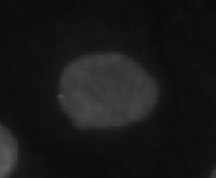
\includegraphics[width=1cm]{img/cell_states_interphase.png} & Interphase & Longest phase, cell nucleus is typically small and convex \\
\hline
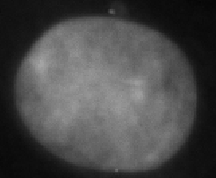
\includegraphics[width=1cm]{img/cell_states_large.png} & Large interphase & Large interphase nucleus, possible replication defect \\
\hline
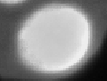
\includegraphics[width=1cm]{img/cell_states_bright.png} & Bright interphase & DAPI at higher intensity, due to cell cycle deregulation \\
\hline
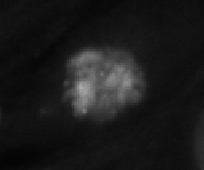
\includegraphics[width=1cm]{img/cell_states_prometaphase.png} & Prometaphase & Mitotic phase, prior to division (short $\implies$ infrequent) \\
\hline
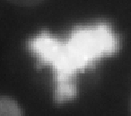
\includegraphics[width=1cm]{img/cell_states_metaphase.png} & Metaphase & Chromosome alignment \\
\hline
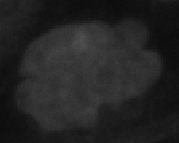
\includegraphics[width=1cm]{img/cell_states_polylobed.png} & Polylobed & Abnormal shape--mitosis abberation \\
\hline
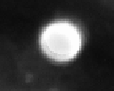
\includegraphics[width=1cm]{img/cell_states_apoptosis.png} & Apoptosis & Cell death \\
\hline
\end{tabular}
\caption{Morphological classes manually annotated on wild type screen data to create a ground truth for training cell classifier.}
\label{table:cell_states}
\end{center}
\end{table}

In order to analyse the morphological landscape of these cell lines, seven nuclear morphology classes have been defined. Table \ref{table:cell_states} lists these classes for the wild type screen: \emph{interphase}, the longest part of the cell cycle, where the cell nucleus is typically small and convex; \emph{large interphase}, corresponding to an abnormally large interphase nucleus, potentially the result of a defect in DNA replication or nuclear membrane control; \emph{bright interphase}, where DAPI exhibits higher fluorescence, presumably due to cell cycle deregulation; \emph{prometaphase}, the first observable mitotic state (condensed chromosomes, broken nuclear envelope), which is relatively rare due to its short duration; \emph{metaphase}, the mitotic phase in which the cell's chromosomes are aligned in the metaphase plate prior to chromosome segregation; \emph{apoptosis}, cell death; and \emph{polylobed}, in which the cell nucleus takes on an abnormal shape, due to problems in the division process.

Phenotypic profiles are not only informative about drug perturbations, but also about cell lines themselves. Indeed, a cancer cell line is supposed to have acquired properties that differentiate them from normal cells. Depending on the markers used, such differences can be measured by imaging approaches. One may hypothesise it to be interesting to identify the phenotypic profiles of the $12$ cancer cell lines from the wild type screen (see Section \ref{subsec:morphogical}), corresponding to different molecular subtypes of TNBC, in order to understand to what extent the molecular subtypes coincide with phenotypic differences. This would allow us to infer the biological processes which are perturbed in these different cell lines.

\begin{figure}[h!]
\centering
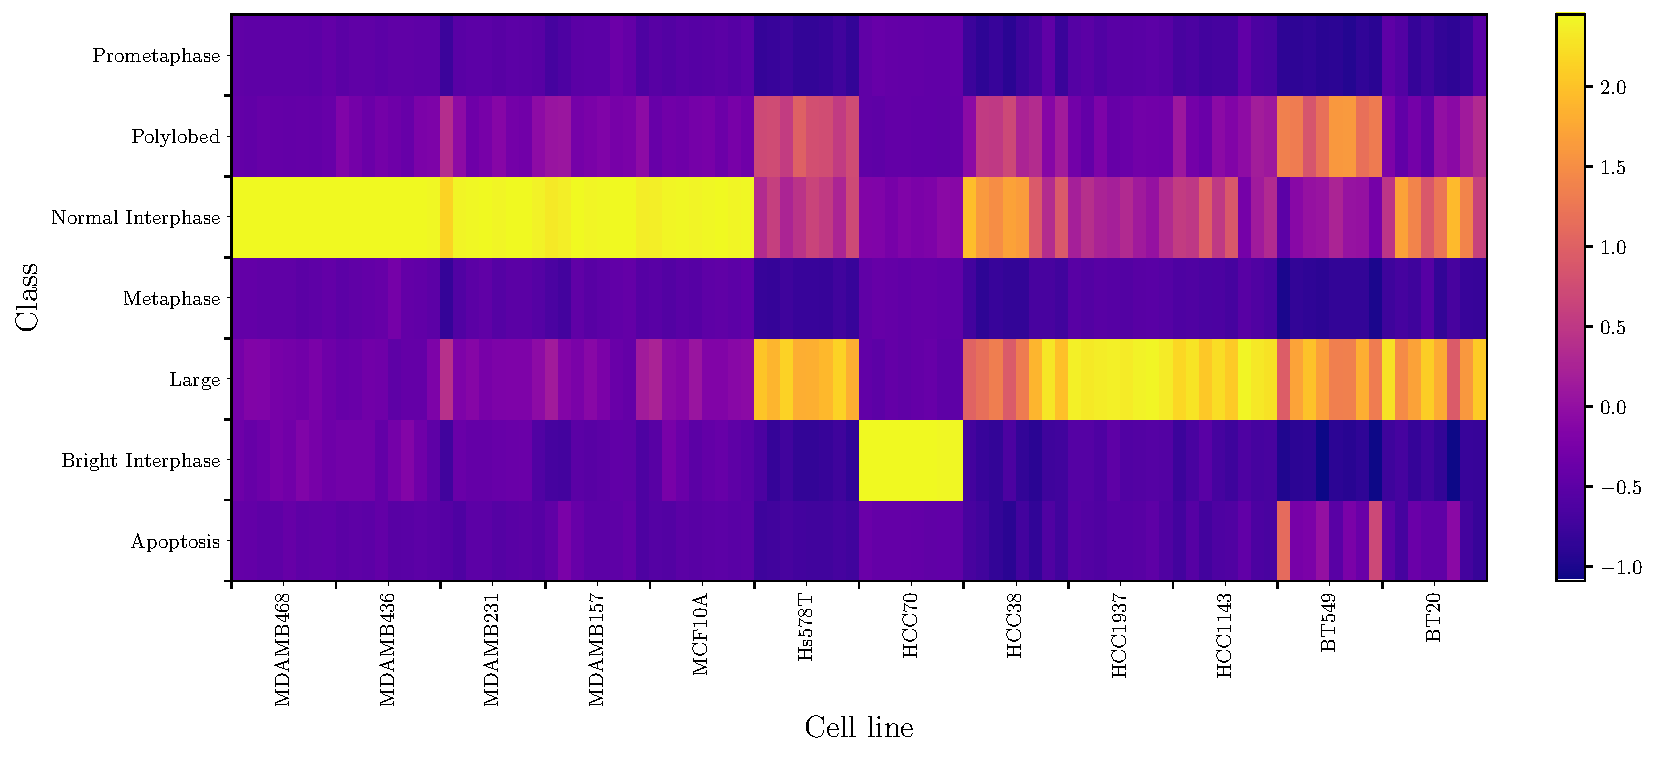
\includegraphics[width=0.95\textwidth]{img/profile.pdf}
\caption{Morphological profiles of $12$ TNBC cell lines with $8$ replicates apiece, based on $7$ biologically meaningful classes, derived from manual annotation. One observes the phenotypic similarity between TNBC families.}
\label{fig:morphological_profiles}
\end{figure}

$926$ cells were annotated in the wild type screen dataset\footnote{Later, a larger set of 6530 cells were annotated and released for pedagogical purposes at https://github.com/jcboyd/deep-learning-workshop/tree/cell-data}, according to seven morphological classes specified in Table \ref{table:cell_states}, from which were extracted the 239 DAPI-channel nuclei features. A SVM with RBF kernel was then trained, with hyperparameters optimised by grid search and $10$-fold cross-validation). The trained SVM was used to classify the remaining cells in the assay (some $36338$ cells in total). The number of cells in each phenotypic class are counted, and divided by the total to create phenotype profiles for each well, that is, a summary of seven proportions for each of the $96$ wells. The profiles were normalised by subtracting the average from the negative control cell line, MCF10A. The $96$ profiles ($8$ per cell line) are visualised in Figure \ref{fig:morphological_profiles}. We can see how families of TNBC cell lines cluster in their phenotypes. Of note are the cell lines of the drug screen, MDA231 and MDA468, which manifest predominantly normal interphase cells.

Figure \ref{fig:umap_cell_lines} plots a (two-dimensional) UMAP dimensionality reduction (\cite{mcinnes2018umap}) of a balanced sample of $150$ cells from $4$ of the $12$ cell lines. We see a clear separation of cell lines in the UMAP embedding, mirroring their distinctive appearance in the microscopy. Note that a subset of cell lines was chosen to avoid clutter, but the same degree of separation was observed across the $12$. The negative control cell line (MCF10A) is included, as is one of the cell lines studied in the drug screen (MDA231).

\begin{figure}[ht]
\centering
\tikzset{every picture/.style={line width=0.75pt}} %set default line width to 0.75pt        

\begin{tikzpicture}[x=0.75pt,y=0.75pt,yscale=-1,xscale=1]
%uncomment if require: \path (0,435); %set diagram left start at 0, and has height of 435

%Image [id:dp32418545643234] 
\draw (157.75,159.75) node  {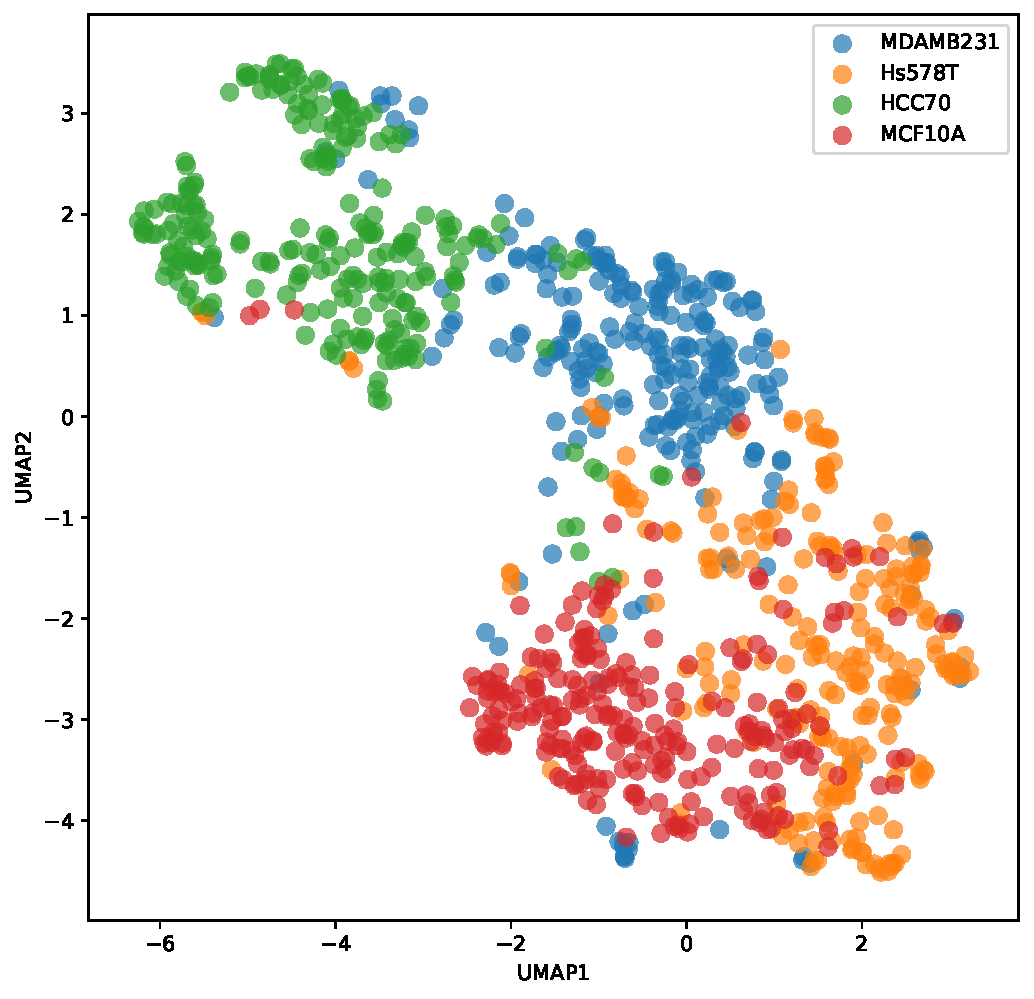
\includegraphics[width=220.13pt,height=220.13pt]{img/tsne_cell_lines.pdf}};
%Image [id:dp04123920029260497] 
\draw (339.5,48) node  {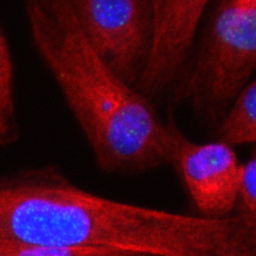
\includegraphics[width=52.5pt,height=52.5pt]{img/tsne_MDAMB231.png}};
%Image [id:dp5038754434164179] 
\draw (339.5,271.5) node  {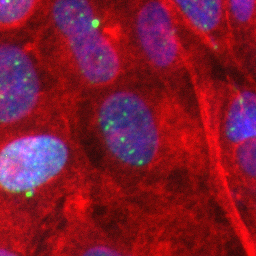
\includegraphics[width=52.5pt,height=52.5pt]{img/tsne_Hs578T.png}};
%Image [id:dp07000232773693138] 
\draw (339.5,196.5) node  {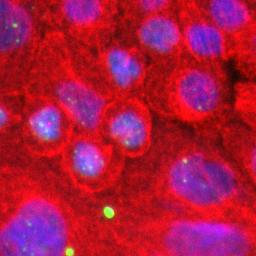
\includegraphics[width=52.5pt,height=52.5pt]{img/tsne_MCF10A.png}};
%Straight Lines [id:da25518923652570036] 
\draw    (303,58) -- (208.88,114.64) ;
\draw [shift={(207.17,115.67)}, rotate = 328.96000000000004] [color={rgb, 255:red, 0; green, 0; blue, 0 }  ][line width=0.75]    (10.93,-3.29) .. controls (6.95,-1.4) and (3.31,-0.3) .. (0,0) .. controls (3.31,0.3) and (6.95,1.4) .. (10.93,3.29)   ;
%Image [id:dp00379357012573478] 
\draw (339.5,122) node  {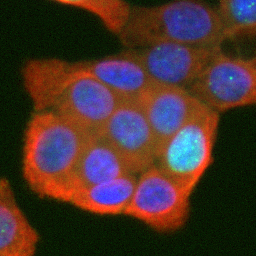
\includegraphics[width=52.5pt,height=52.5pt]{img/tsne_HCC70.png}};
%Straight Lines [id:da7273031760959292] 
\draw    (304,124) -- (129.12,87.08) ;
\draw [shift={(127.17,86.67)}, rotate = 371.91999999999996] [color={rgb, 255:red, 0; green, 0; blue, 0 }  ][line width=0.75]    (10.93,-3.29) .. controls (6.95,-1.4) and (3.31,-0.3) .. (0,0) .. controls (3.31,0.3) and (6.95,1.4) .. (10.93,3.29)   ;
%Straight Lines [id:da2435407636909176] 
\draw    (304,198) -- (259.13,207.26) ;
\draw [shift={(257.17,207.67)}, rotate = 348.34000000000003] [color={rgb, 255:red, 0; green, 0; blue, 0 }  ][line width=0.75]    (10.93,-3.29) .. controls (6.95,-1.4) and (3.31,-0.3) .. (0,0) .. controls (3.31,0.3) and (6.95,1.4) .. (10.93,3.29)   ;
%Straight Lines [id:da4514217956323979] 
\draw    (303,271) -- (165.05,222.33) ;
\draw [shift={(163.17,221.67)}, rotate = 379.43] [color={rgb, 255:red, 0; green, 0; blue, 0 }  ][line width=0.75]    (10.93,-3.29) .. controls (6.95,-1.4) and (3.31,-0.3) .. (0,0) .. controls (3.31,0.3) and (6.95,1.4) .. (10.93,3.29)   ;
\end{tikzpicture}
\caption{UMAP projection from feature space of sample cells from four TNBC cell lines (selected among 12) in a wild type screen. On the right we show a fixed-size ($128\times128$px) crop centered on an indicative cell from each cell line.}
\label{fig:umap_cell_lines}
\end{figure}

A random forest classifier with $500$ trees is also trained to classify cell lines in feature space. The data set is built from a balanced sampling of $150$ cells per cell line, totaling $1800$ cells, with $25\%$ of the data reserved for testing. The random forest achieves in excess of $70\%$ accuracy on the $450$ test samples. A confusion matrix is provided in Appendix \ref{AppendixA}. Repeated experiments reveal that the greatest confusion occurs between two cell lines of the same family: MDA231 and MDA436. Thus, even with a small fraction of the total data available for training (and little to no tuning), an off-the-shelf classifier achieves a strong accuracy. This demonstrates that the cells of distinct cell lines occupy different regions of the feature space and that their wild type morphologies are different.

In this section we have seen two levels of phenotypic distinction between TNBC cell line wild types. The first concerns the regulation of cell states, as in Figure \ref{fig:morphological_profiles}, where we saw how cell populations over different cell lines could be differentiated in a morphological profile, which appeared to cluster by pathology. Through annotation (first manual, then by classifier), these morphological classes abstracted away from the second distinction, that of the morphology of individual cells within each cell line, as in Figure \ref{fig:umap_cell_lines}. It is overcoming this second distinction that will play a strong role in the motivations of the methods of Chapter \ref{Chapter4}, albeit in an unsupervised setting where manual annotation is not feasible.

%\begin{figure}
%\centering
%\resizebox{8cm}{8cm}{
%\begin{tikzpicture}
%
%\def\radius{3}
%
%\filldraw[fill={rgb,255:red,255; green,237; blue,187}, line width=1]
%(0,0)--plot[domain=-pi/8:pi/2] (xy polar cs:angle=\x r, radius=\radius)--cycle;  % cycle connects path back to the origin
%\node[font=\LARGE] at (3*pi/16r : 3.5) {G1};  % draw digits -- r for radians in polar coordinates
%
%\filldraw[fill={rgb,255:red,181; green,209; blue,237}, line width=1]
%(0,0)--plot[domain=pi/2:5*pi/8] (xy polar cs:angle=\x r, radius=\radius)--cycle;
%\node[font=\LARGE] at (9*pi/16r : 3.5) {M};  % draw digits -- r for radians in polar coordinates
%
%\filldraw[fill={rgb,255:red,255; green,207; blue,141}, line width=1]
%(0,0)--plot[domain=5*pi/8:9*pi/8] (xy polar cs:angle=\x r, radius=\radius)--cycle;
%\node[font=\LARGE] at (7*pi/8 r:3.5) {G2};  % draw digits -- r for radians in polar coordinates
%
%\filldraw[fill={rgb,255:red,197; green,223; blue,155}, line width=1]
%(0,0)--plot[domain=9*pi/8:15*pi/8] (xy polar cs:angle=\x r, radius=\radius)--cycle;
%\node[font=\LARGE] at (12*pi/8 r:3.5) {S};  % draw digits -- r for radians in polar coordinates
%
%% draw arrow
%\node[font=\LARGE] at (3*pi/8r : {1.25*\radius}) {time};  % draw digits -- r for radians in polar coordinates
%\draw[->, line width=1] plot[domain=pi/2:pi/4] (xy polar cs:angle=\x r, radius={1.1*\radius});
%
%\end{tikzpicture}
%}
%\caption{Cell cycle phases of a human cell line (24 hours: G1 = 11; S = 8; G2 = 4; M = 1). Inspired by \cite{cooper2004cell}.}
%\label{fig:cycles}
%\end{figure}



% We then compare each of these profiles to each of the 41556 profiles in the Mitocheck dataset. We use cosine distance to rank the closest profiles, giving a list of candidates for silenced genes. The final step is to compare this prediction with gene expression data of the same cell line. Should it be that the prediction matches, we will have discovered a way of prioritizing candidate genes from image data.
%
%Moreover, we will compare the phenotypic profiles from the TNBC cell lines with an existing genome-wide RNA interference (RNAi) screen \emph{Mitocheck} \cite{neumann2010phenotypic}. RNAi is a process by which genes can be prevented from being expressed by degradation of the corresponding mRNA. This is also known as ``gene silencing''. A genome-wide RNAi screen contains the phenotypic responses to silencing each individual gene in the genome. Our hope is that if we can compare the cell lines at the phenotypic level with a genome-wide RNAi screen, we can check which gene silencing experiments lead to similar phenotypes as the wild-type experiments. We can then combine this information with gene expression profiles for the cell lines in order to give higher priority to those candidates that are both downregulated in the cell lines (as compared to normal cell lines) and whose phenotype in RNAi data is consistent with the cell line phenotype we observe. This strategy is illustrated in Figure \ref{fig:flowchart}.

%\tikzstyle{block} = [rectangle, draw, fill=blue!20, node distance=3cm,
%    text width=5em, text centered, rounded corners, minimum height=4em]
%\tikzstyle{line} = [draw, -latex']
%
%\begin{figure}
%\begin{tikzpicture}[node distance = 2cm, auto]
%    % Place nodes
%    \node [block, fill=red!20] (features) {Extracted features};
%    \node [block, below of=features] (norm) {Dim. reduction};
%    \node [block, right of=norm] (kmeans) {K-means};
%    \node [block, right of=kmeans] (subsample) {Balanced subsample};
%    \node [block, right of=subsample] (cluster) {Clustering};
%    \node [block, above right of=cluster] (visualise) {Visualise t-SNE};
%    \node [block, below right of=cluster] (crops) {Sample crops};
%    % Draw edges
%    \path [line] (features) -- (norm);
%    \path [line] (norm) -- (kmeans);
%    \path [line] (kmeans) -- (subsample);
%    \path [line] (subsample) -- (cluster);
%    \path [line] (cluster) -- (visualise);
%    \path [line] (cluster) -- (crops);
%\end{tikzpicture}
%\caption{Pipeline for class discovery.}
%\end{figure}

%\begin{figure}
%\begin{tikzpicture}[node distance=2cm, auto]
%    % Place nodes
%    \node [block, fill=red!20] (annotation) {Manual annotation};
%    \node [block, right of=annotation] (train) {Train classifier};
%    \node [block, right of=train] (classify) {Classify};
%    \node [block, right of=classify] (profile) {Compute profiles};
%    \node [block, right of=profile] (nn) {Nearest neighbour};
%    \node [block, below of=nn, fill=red!20] (mitocheck) {Mitocheck data};
%    \node [block, above of=nn, fill=red!20] (expression) {Expression data};
%    % Draw edges
%    \path [line] (annotation) -- (train);
%    \path [line] (train) -- (classify);
%    \path [line] (classify) -- (profile);
%    \path [line] (profile) -- (nn);
%    \path [line] (mitocheck) -- (nn);
%    \path [line] (expression) -- (nn);
%\end{tikzpicture}
%\caption{Flowchart for phenotypic profiling.}
%\end{figure}

